This chapter provides detailed specifications of the system under development.

\section{Functional Requirements}

This section describes each function/feature provided by our system. These functions are logically grouped into modules based on their purpose/users/mode of operations etc (as per our system):
\begin{outline}
  \subsection{Web Application}
  \1 Allows customers to upload a photo of an outfit.
  \1 Displays constituent items of uploaded outfit.
  \1 Allows customers to click on a constituent item and view items identical/similar to it.
  \1 Allows customers to click on an item and open it's product page.
  \1 Displays item title, description, price, photos and sizes on product page.
  \1 On the product page, displays recommendations for similar products, as received from the recommendation engine.
  \1 On the product page, displays recommendations for complementary products, as received from the recommendation engine.
  \1 Allows customer to add item to cart.
  \1 Allows new customers to sign-up.
  \1 Allows returning customers to login.
  \1 Saves user history to database.
  \1 For existing customers with a user history: Displays recommendations based on user history, as received from the recommendation engine, on the home page.
  \1 For existing customers with a user history: Displays recommendations based on user history, as received from the recommendation engine, on product pages.
  \1 For new customers or existing customers without user history: Displays items currently trending on the store, on the home page.
  \1 Admin has exclusive access to an admin panel that allows them to add, remove and modify items on the website. 
  \1 Admin can view customer activity.
\end{outline}
\begin{outline}
  \subsection{Recommendation Engine}
  The engine can be roughly compartmentalized as follows:
  \1 On uploaded photo, calls feature extraction model and performs multiple object detection. To bounding boxes of each individual piece of clothing in the outfit.
  \1 Crops each bounding box in image and returns them. Each bounding box represents an article of clothing.
  \1 Upon receiving which bounding box has been selected by the user, it passes that to nearest neighbour model. Returns ids of n closest neighbours of that item from the database and ids of n best complimentary items.
\end{outline}
\begin{outline}
  \subsection{Database}
  \1 Should store id, title, price, description, sizes, category and tags for each item.
  \1 Should store user and admin account information.
  \1 Should store user profile information, including past logs, search history, purchase history, as well as other related actions.
\end{outline}
\begin{outline}
  \subsection{Web Scraper}
  \1 Crawl local fashion stores `Furor', `Export Leftovers', `J.', `Zellbury', etc.
  \1 For each item of men's clothing on the store, save the photo, description and price locally.
  \1 Add timed cron job functionality so that the database can be verified and kept up to date without discrepancies.
\end{outline}

\section{Non-functional Requirements}

\subsection{Performance Requirements}

\begin{itemize}
    \item High performance of the computer on which the server is hosted is needed to cater to thousands of users. 
    
    \item Fetching the dashboard to view information and recommended outfits shall take no longer than 5 seconds.
\end{itemize}

\subsection{Safety Requirements}
\begin{itemize}
    \item The system must not halt or lag, especially during the update time and must not go down under high traffic. In order to ensure safety of the server, it is suggested that it is hosted on two computers - one kept as a backup.
\end{itemize}

\subsection{Security Requirements}
\begin{itemize}
    \item It must be ensured that only the authorized admins, with valid user credentials, have access to the data of the users in order to ensure user privacy. 
    
    \item The system will use databases from authentic sources and fashion stores.
\end{itemize}

\subsection{User Interface}
\begin{itemize}
    \item The UI/UX flow needs to be intuitive as well as modern. 
\end{itemize}

\subsection{Error Handling}
\begin{itemize}
    \item The system prevents data loss by carefully handling all expected and non-expected errors. 
\end{itemize}

\section{External Interfaces}

\subsection{User Interfaces}

\subsubsection{Customer Interface}

\FloatBarrier
\begin{outline}
  \1 Homepage
  
  This interface would be visible to all the users and would lead to multiple other interfaces such as Login, Clothing categories, User profile, etc. This is shown in \autoref{gui:home}.


    
  \1 Registration
  
  This page allows a new user to create an account by filling the mandatory fields of 'User Name', 'Email', 'Password' and 'Confirmed Password'. In case of valid details, user will be able to login, else they are redirected to the same sign-up page. This is shown in \autoref{gui:sign}.


    
  \1 Login
  
  This interface enables user to log into the system using valid credentials, and redirects him/her to the homepage if the credentials are validated, otherwise an error message is displayed. Login interface requires 'User Name' and 'Password' as the mandatory fields. This is shown in \autoref{gui:login}.


  \1 Profile
  
  A user would be able to see this interface if they have created an account and are logged into the system. This interface would enable them to view their account details and their previously searched/recommended outfit statistics. This is shown in \autoref{gui:profile}.


  \1 Product Display
  
  A user would be able to see different product categories along with the details of each product available in the stock. This is shown in \autoref{gui:product1}, \autoref{gui:product2}, and \autoref{gui:product3}.
  

  
  
  \1 Upload Image
  
  A user would be able to upload image of his/her clothing item, in order to search visually similar or complementary items. This is shown in \autoref{gui:upload1} and \autoref{gui:upload2}.
  


  \1 Cart
  
  This interface enables a user to view their selected recommended outfits and would show them the third-party referral links to each of their chosen outfits. This is shown in \autoref{gui:cart}.
  

  \1 Our Brands

  This interface would display the vendors and the third-party brands with whom we will partner up with. A user would be able to retrieve products based on any specific store from these brands. This is shown in \autoref{gui:brands}. 
  
 \end{outline}
 
 \subsubsection{System Admin Interface}
 \begin{outline}
   \1 Login
   
   Using the login interface, the system admin would log into the system using his/her valid credentials and would be redirected to the system admin homepage. This is shown in \autoref{gui:login}.
   
   \1 Homepage
   
   This interface enables the system admin to get redirected to multiple other navigation pages such as User Details, and Vendor details. This is shown in \autoref{gui:home}.
   
   \1 User Details
   
   This interface contains user details such as their personal information, their cart details and their preferred trend statistics. This is shown in \autoref{gui:profiles1} and \autoref{gui:profiles2}.
   
   \1 Vendor Details
   
   This interface allows the system admin to view details of the vendor such as the trends of their most recommended outfits, new additions to their outfit database, top users visiting the respective vendor page (using the referral link). This is shown in \autoref{gui:vendor1} and \autoref{gui:vendor2}.
 \end{outline}

\subsubsection{GUI Mockups}
\begin{figure}[H]
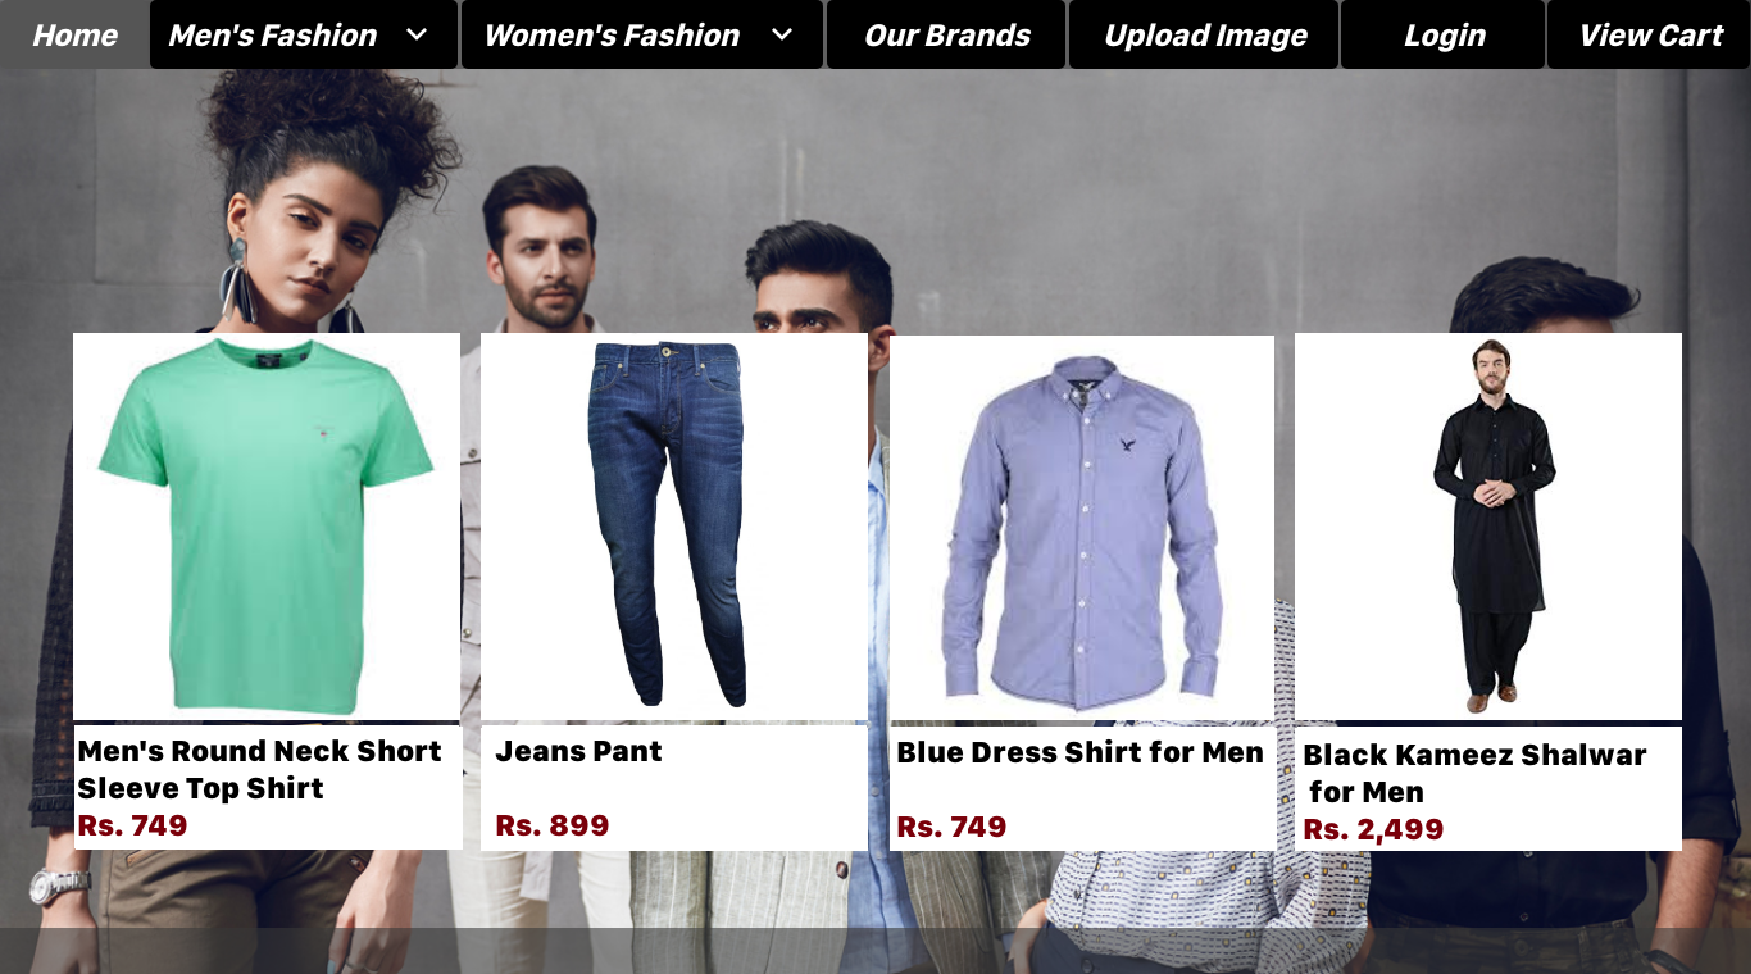
\includegraphics[width=15cm]{images/HomeScreen.pdf} 
\centering
\caption{Home Screen}
\label{gui:home}
\end{figure}

 \begin{figure}[H]
  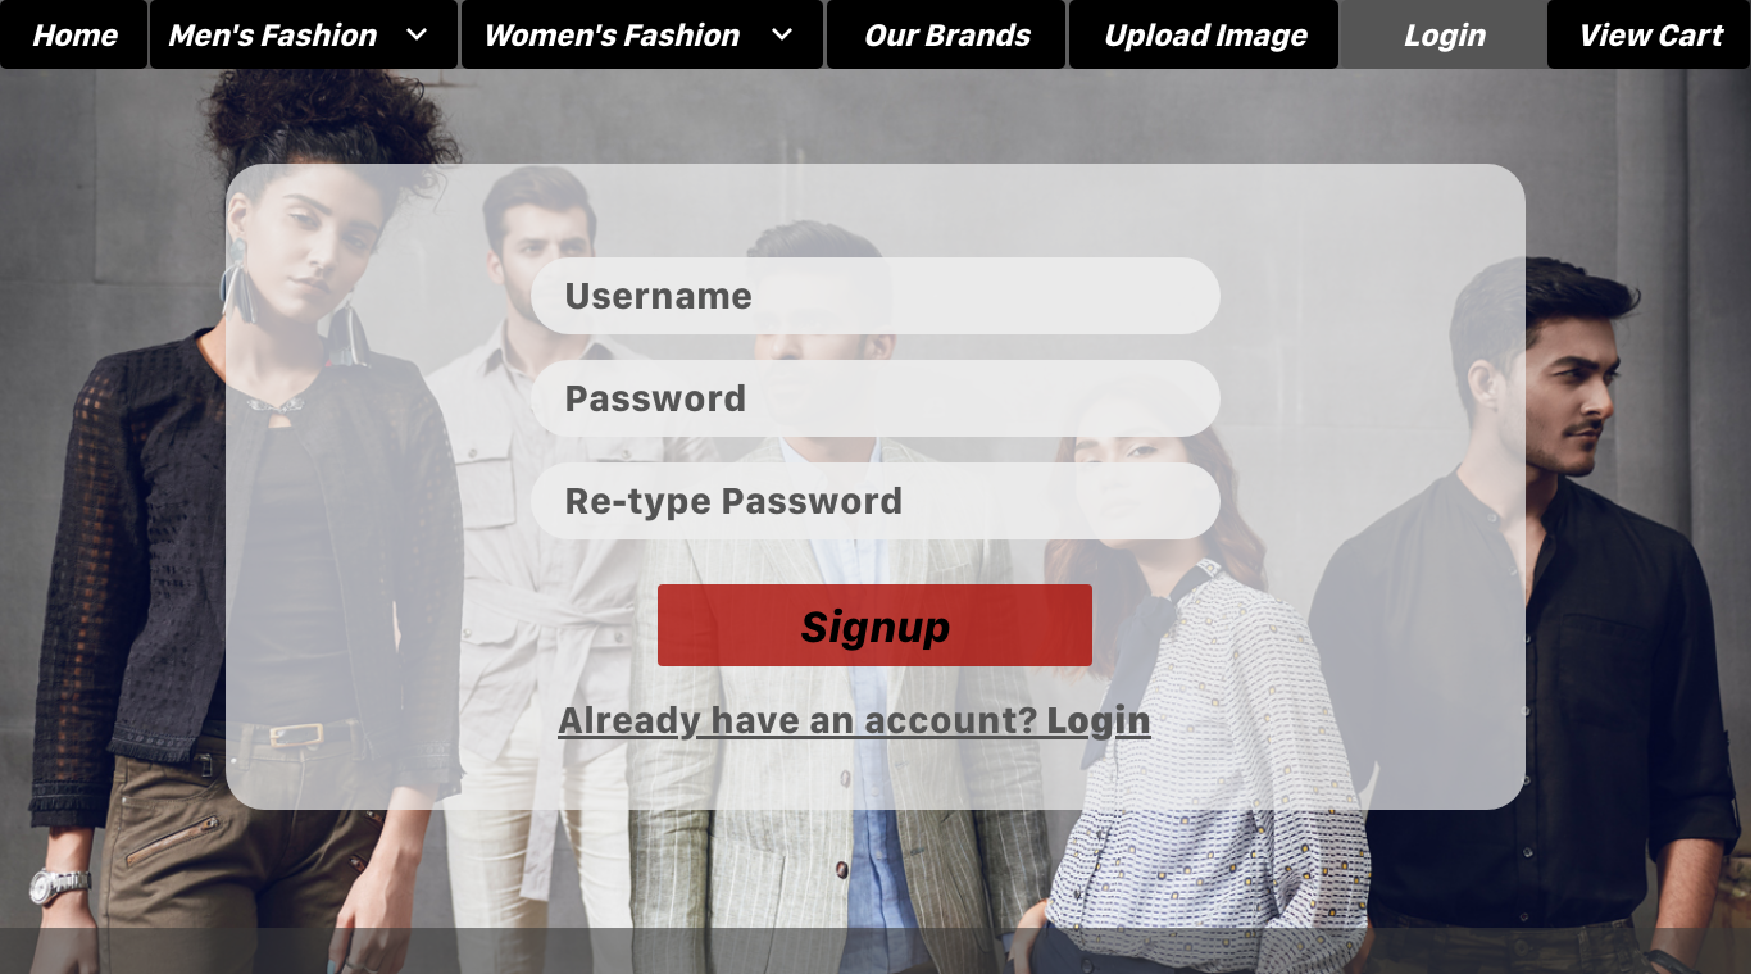
\includegraphics[width=15cm]{images/SignupScreen.pdf} 
  \centering
  \caption{Sign-up Screen}
  \label{gui:sign}
  \end{figure}

  \begin{figure}[!htb]
  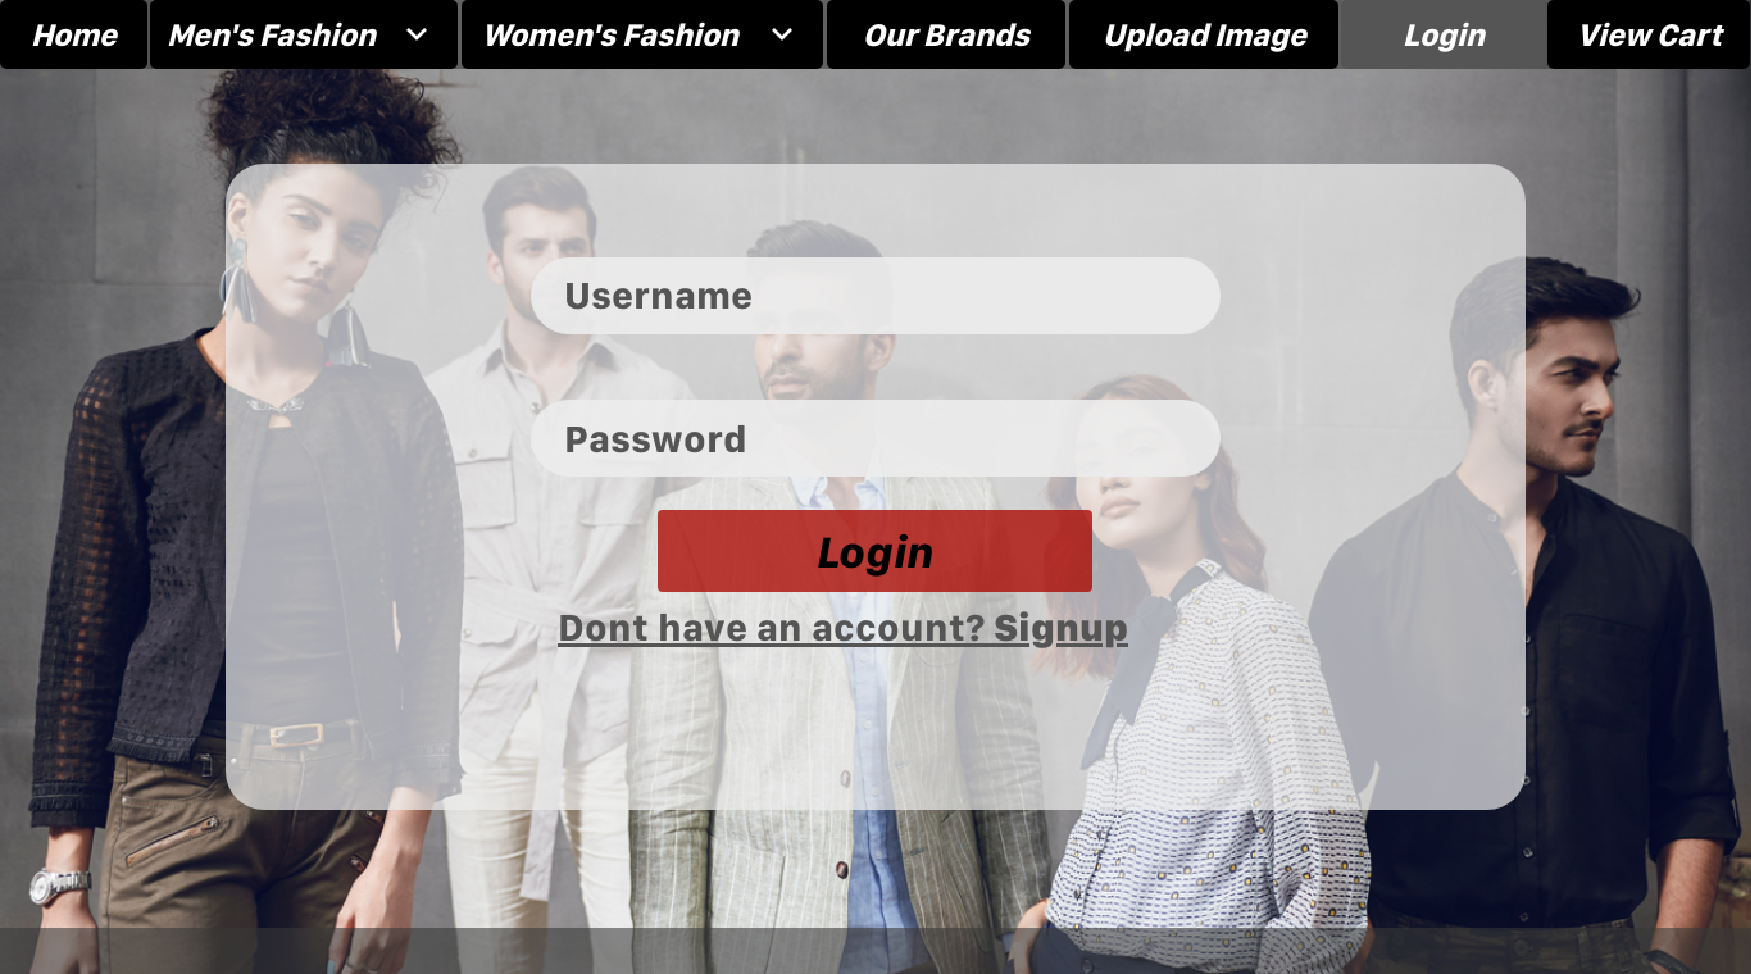
\includegraphics[width=15cm]{images/LoginScreen.pdf} 
  \centering
  \caption{Login Screen}
  \label{gui:login}
  \end{figure}

  \begin{figure}[H]
  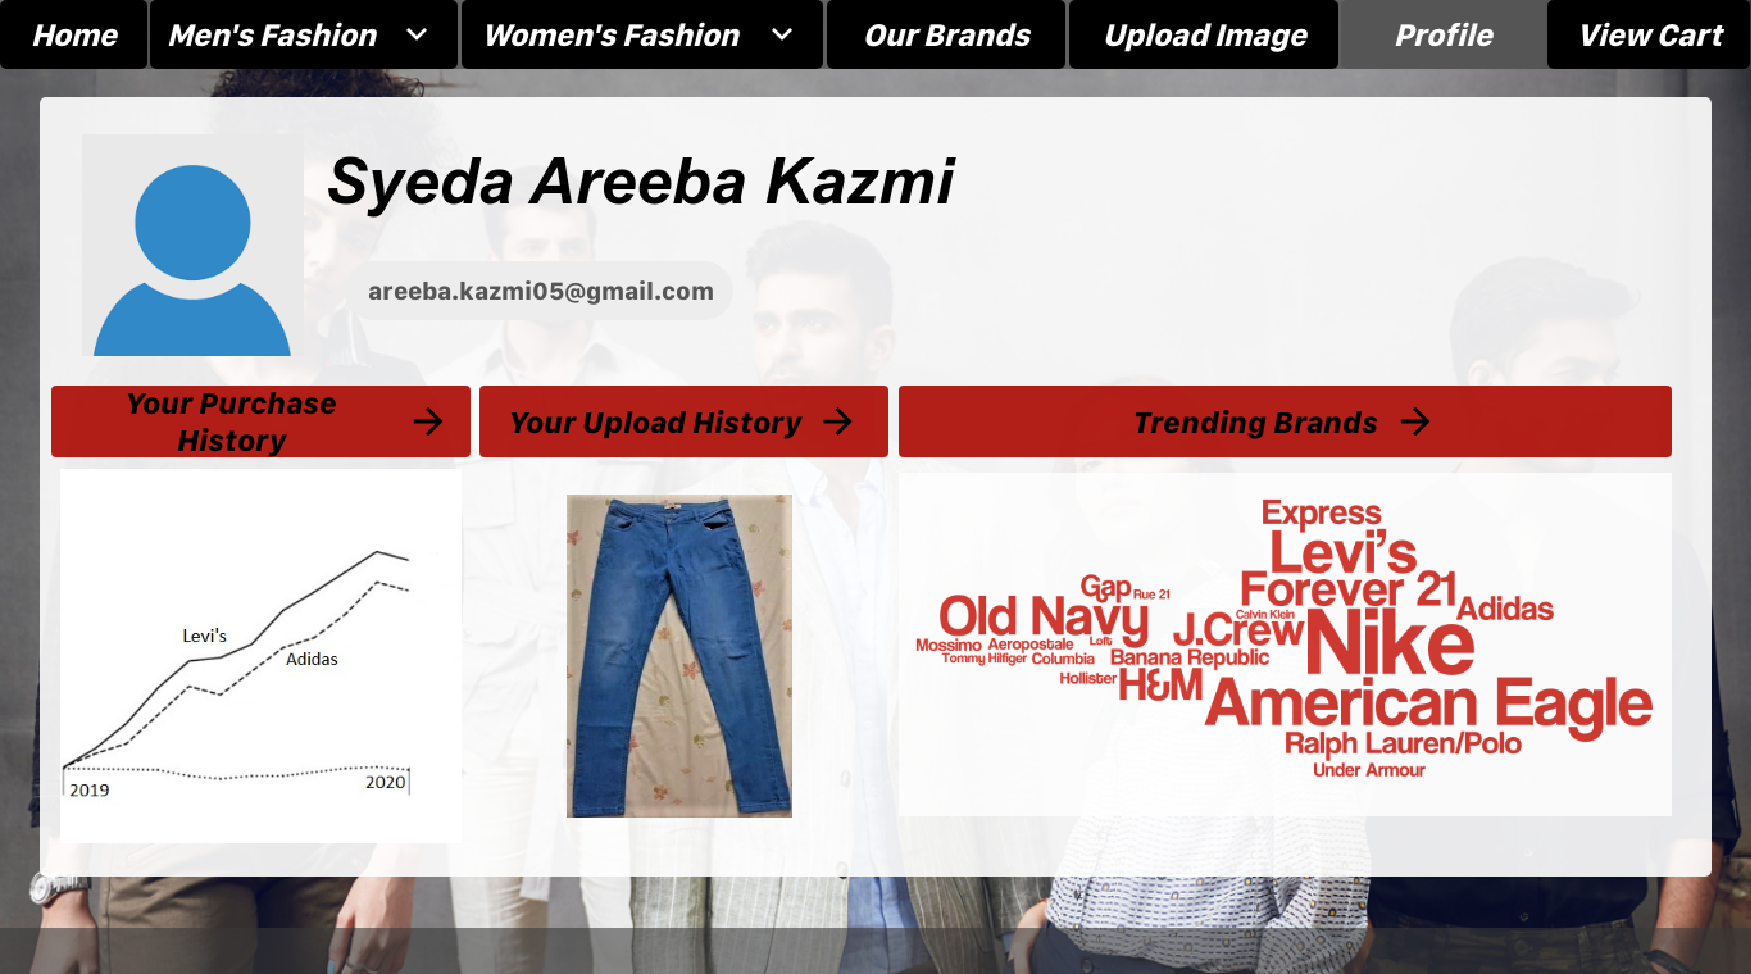
\includegraphics[width=15cm]{images/UserProfileScreen.pdf} 
  \centering
  \caption{User Profile Screen}
  \label{gui:profile}
  \end{figure}
  \begin{figure}[H]
  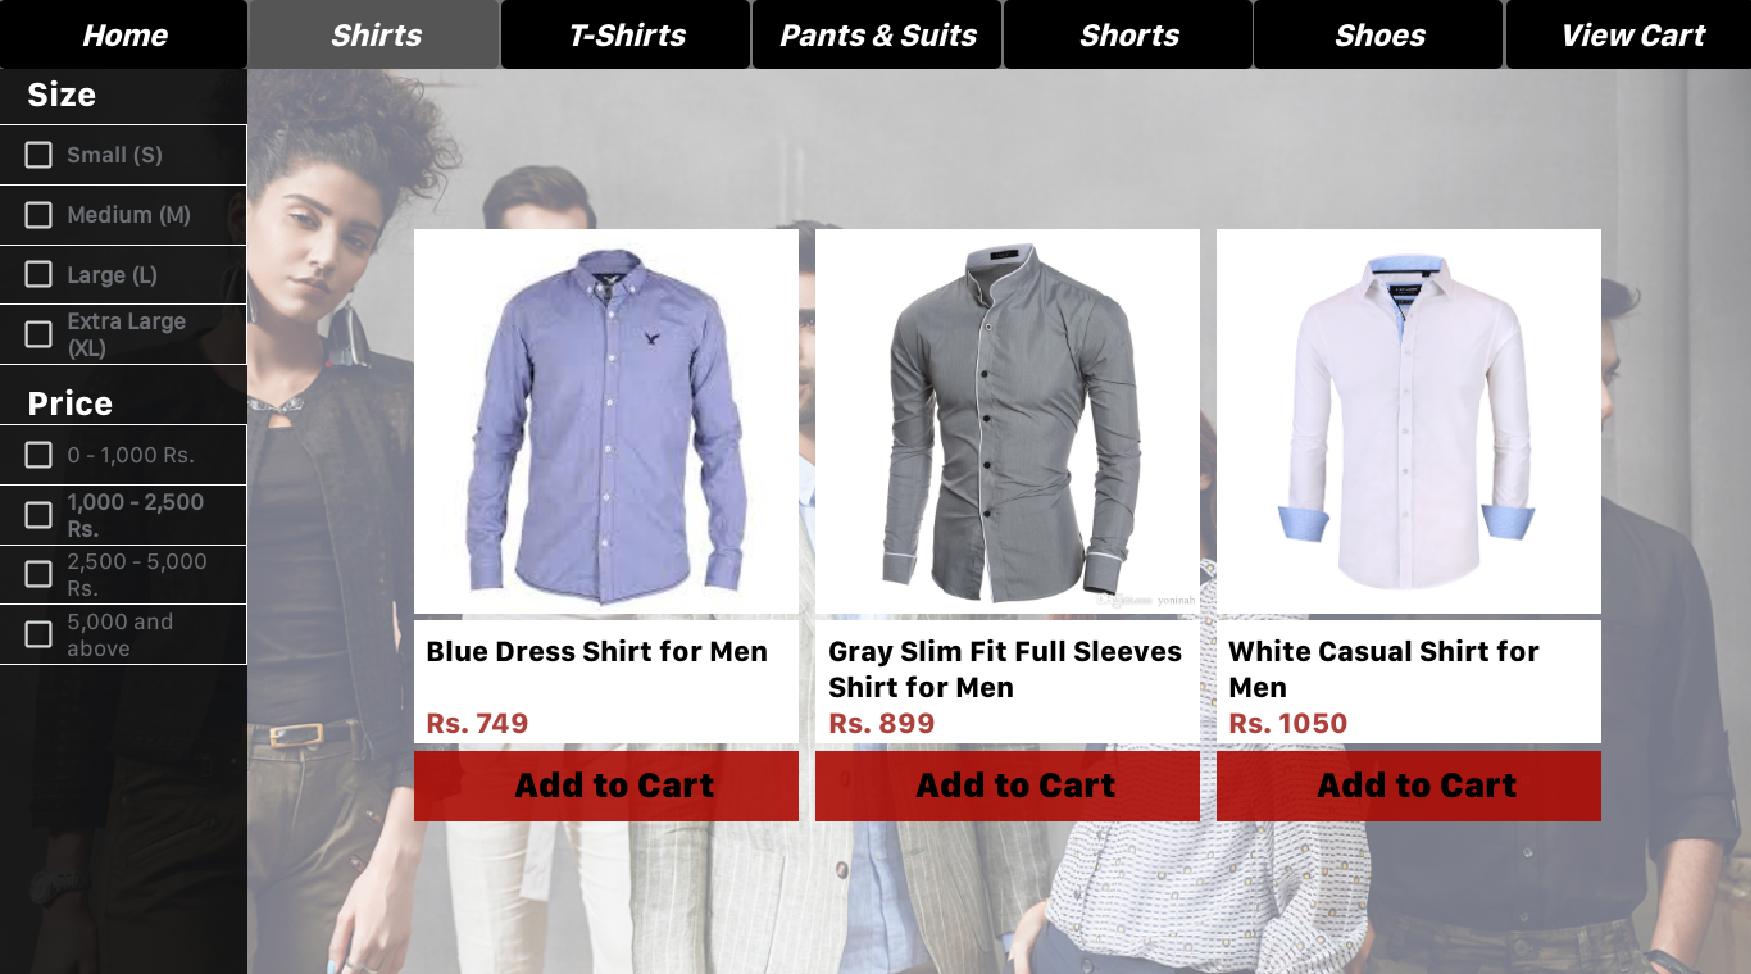
\includegraphics[width=15cm]{images/ShirtsScreen.pdf} 
  \centering
  \caption{Shirt Category Screen}
  \label{gui:product1}
  \end{figure}
  
  \begin{figure}[H]
  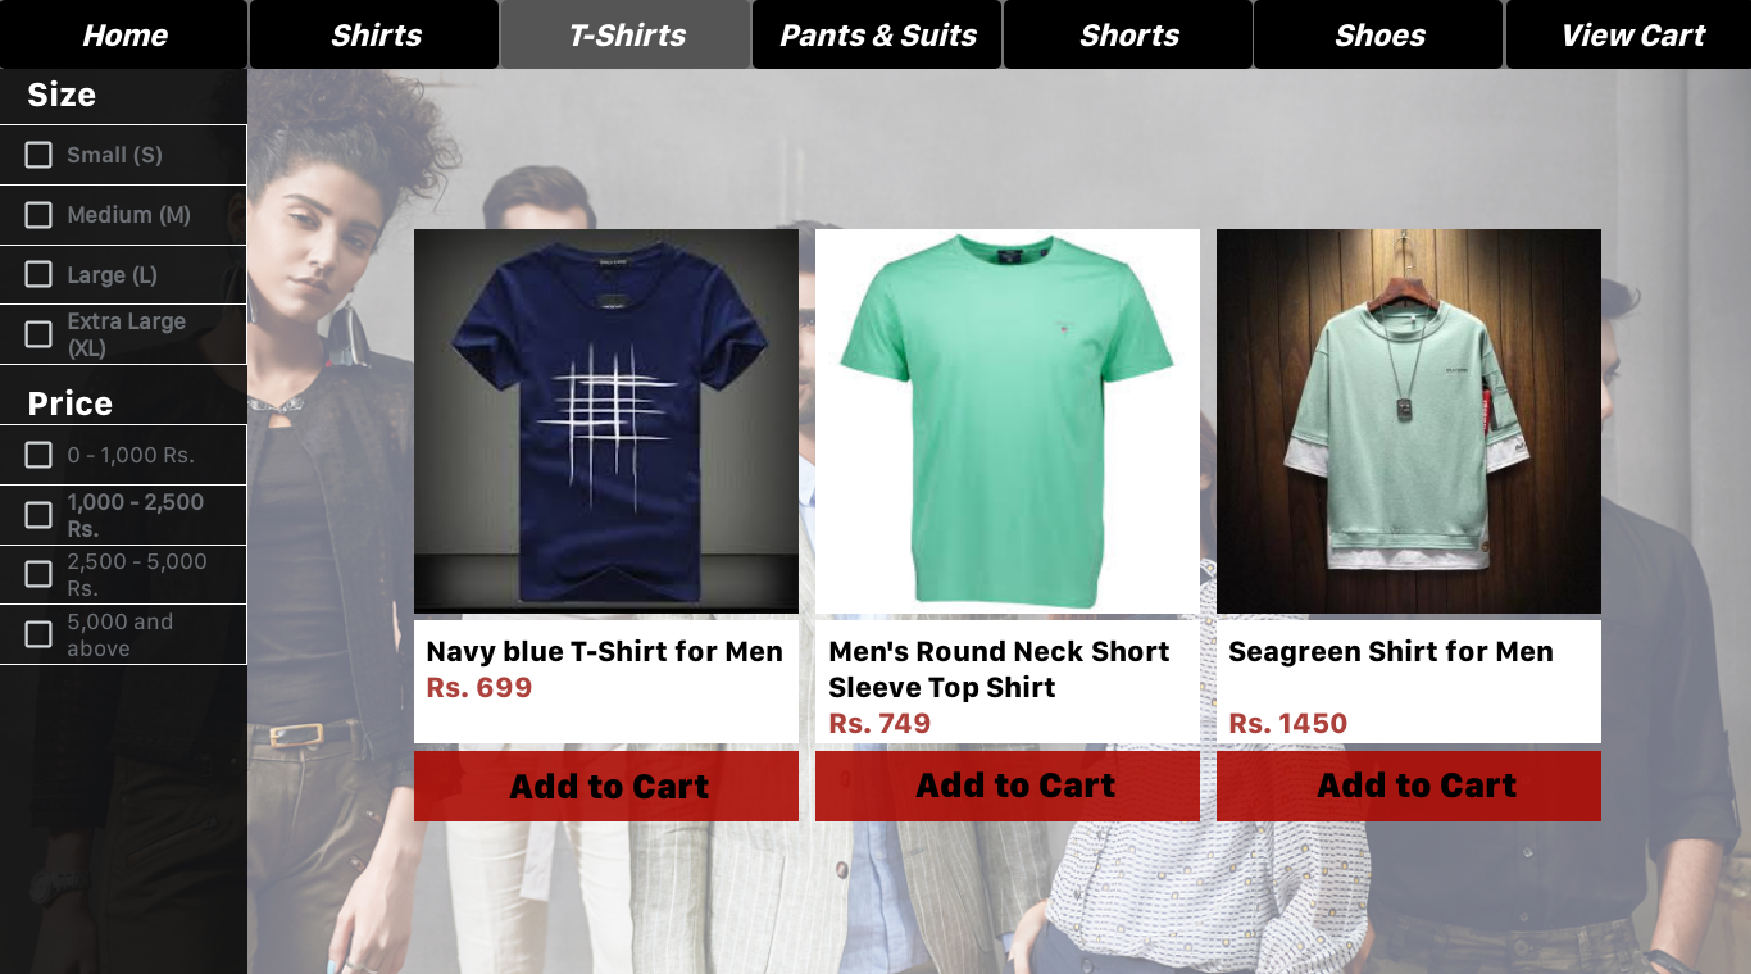
\includegraphics[width=15cm]{images/TShirtsScreen.pdf}
  \centering
  \caption{T-Shirt Category Screen}
  \label{gui:product2}
  \end{figure}
  
  \begin{figure}[H]
  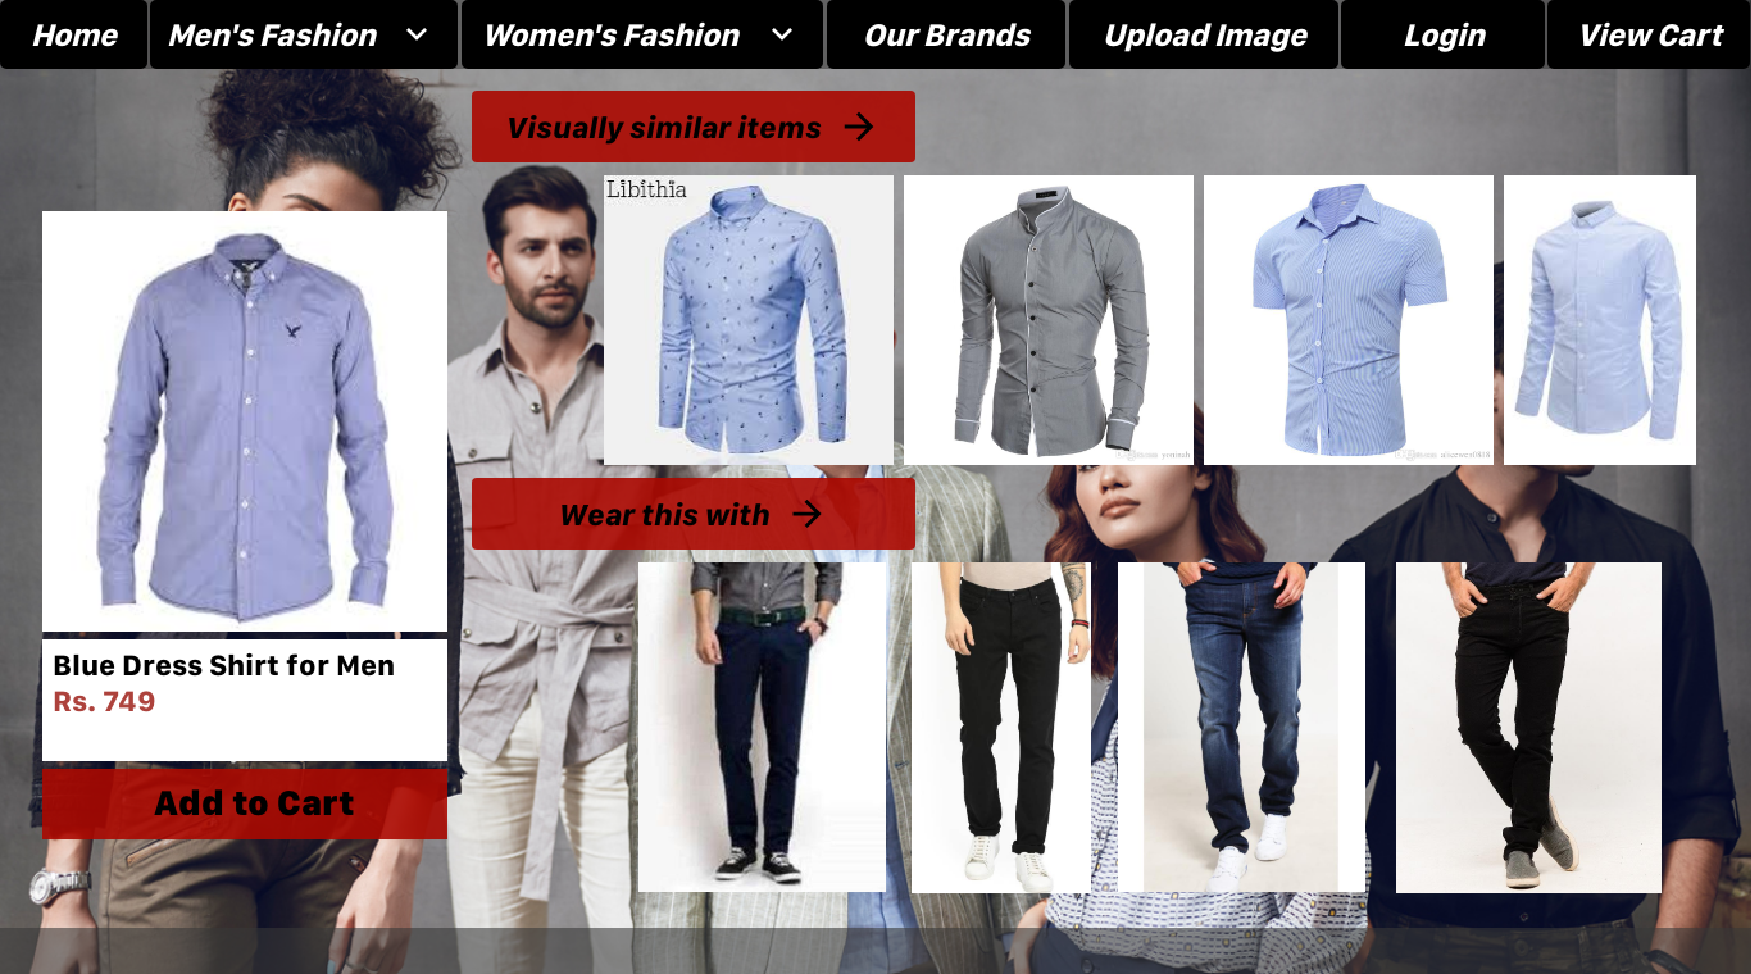
\includegraphics[width=15cm]{images/ProductDetailsScreen.pdf} 
  \centering
  \caption{Recommendation Screen 1.0}
  \label{gui:product3}
  \end{figure}
  \begin{figure}[H]
  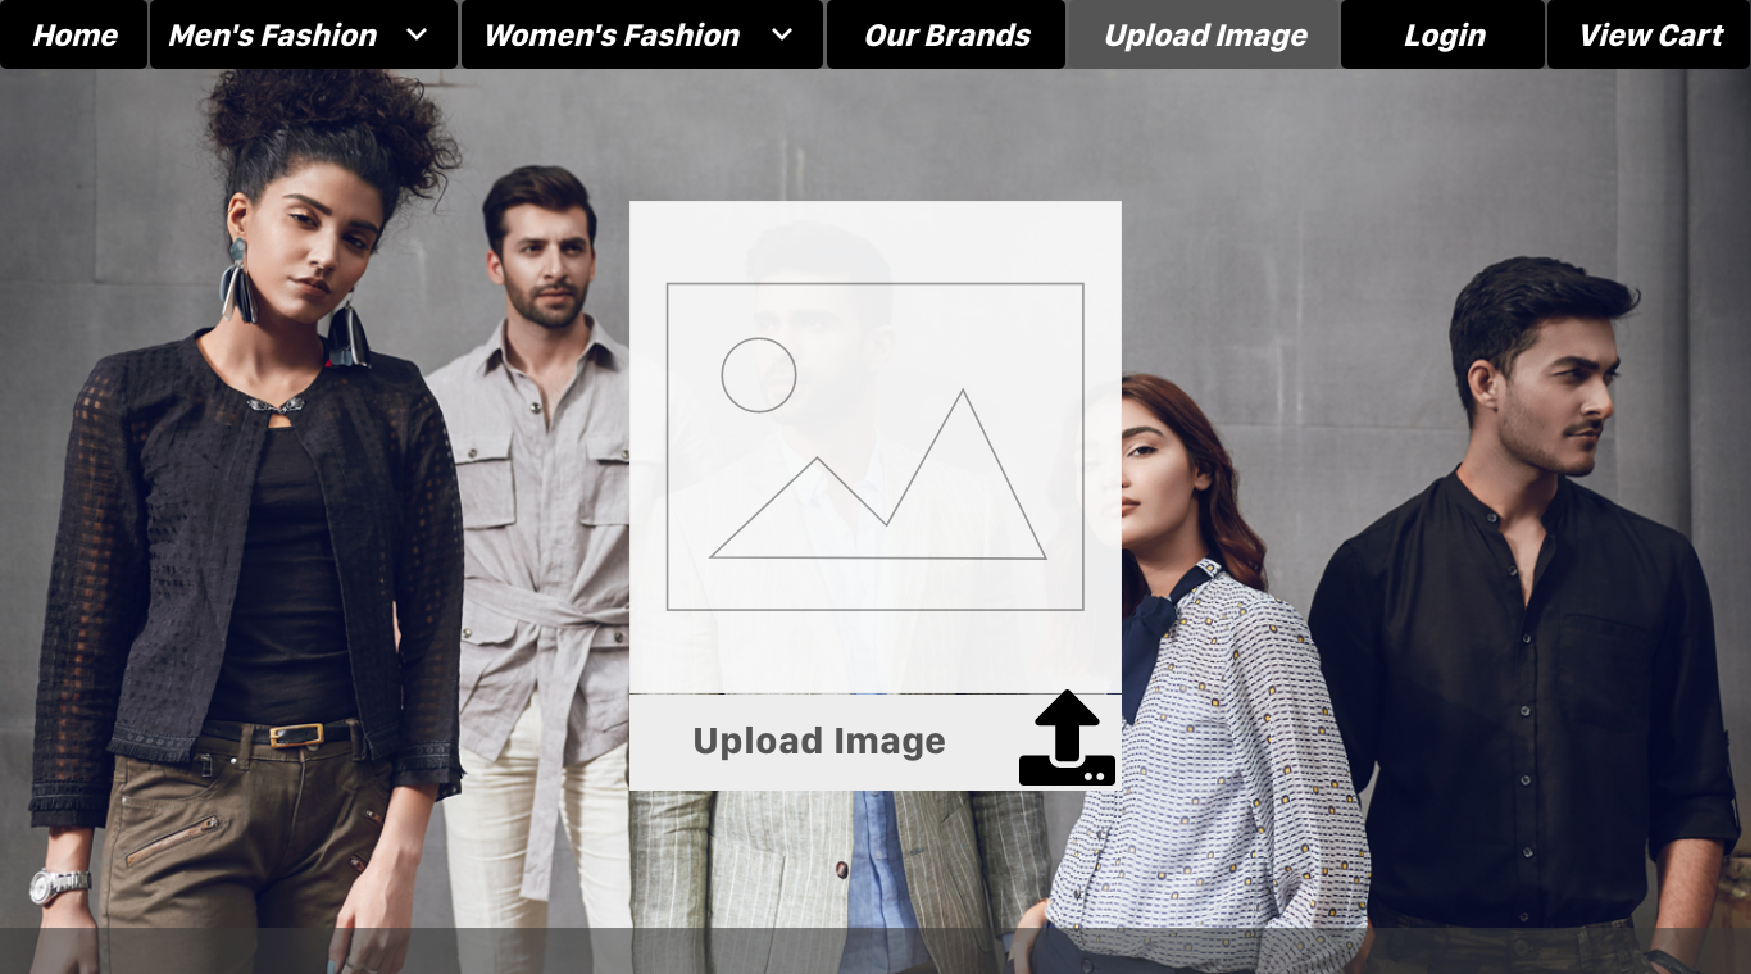
\includegraphics[width=15cm]{images/UploadImageScreen.pdf} 
  \centering
  \caption{Upload Image Screen}
  \label{gui:upload1}
  \end{figure}
  
  \begin{figure}[H]
  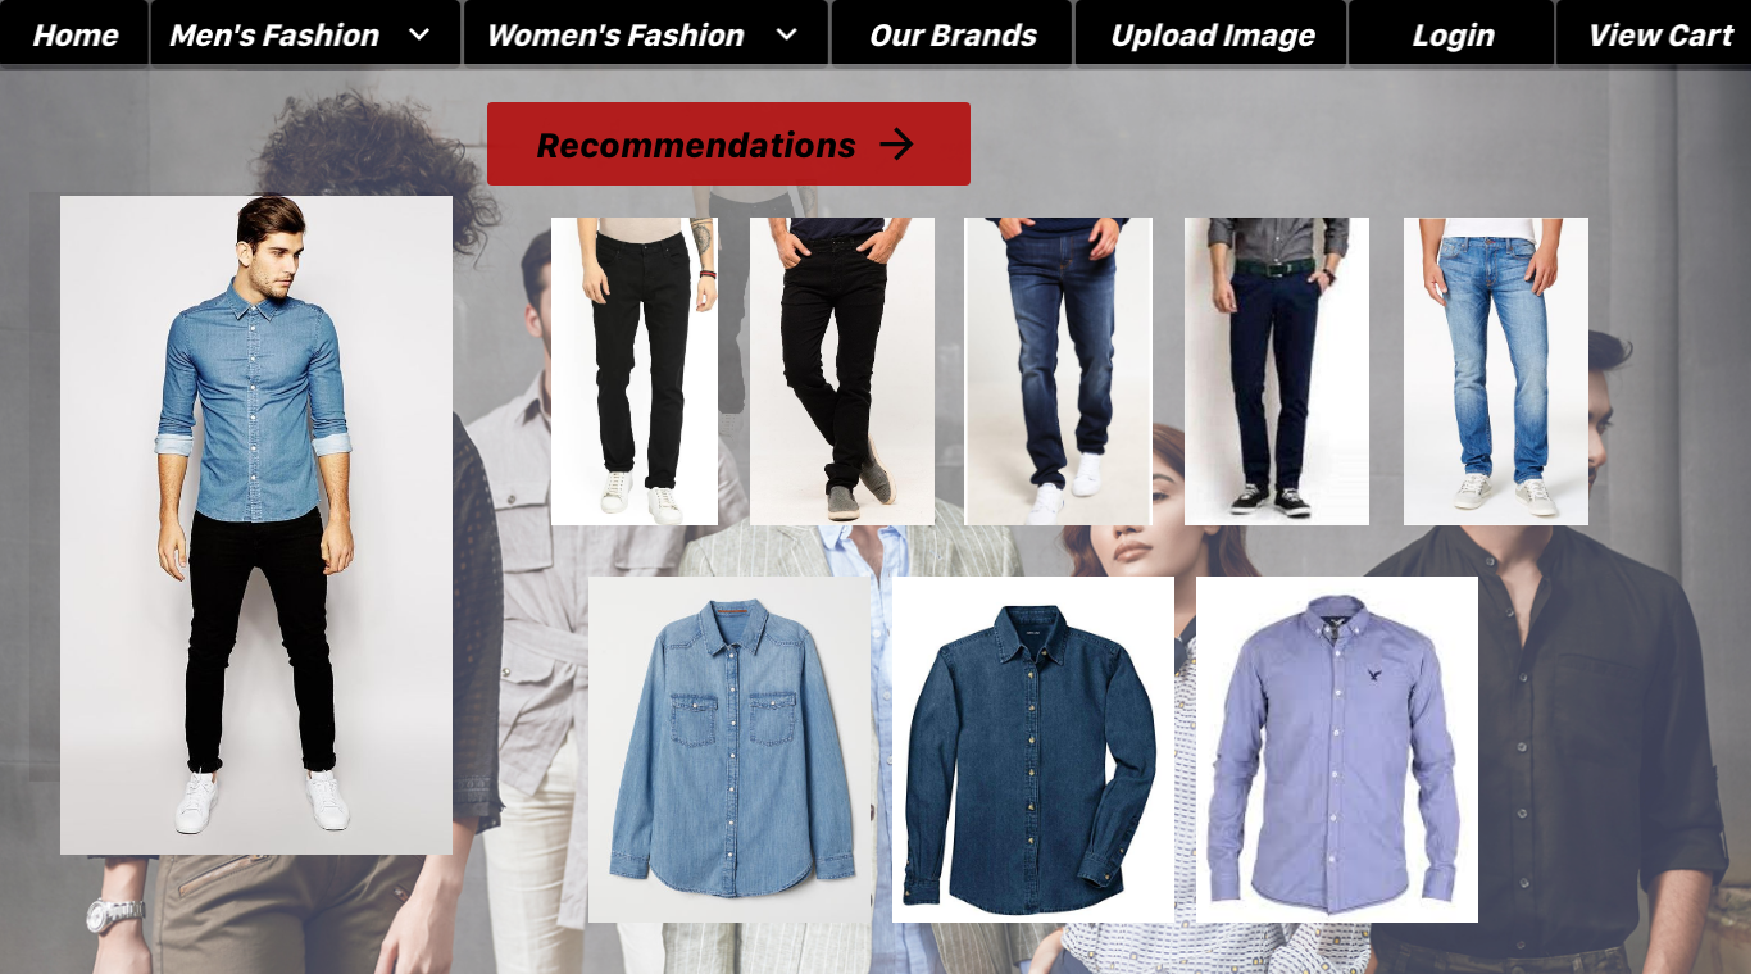
\includegraphics[width=15cm]{images/UploadedImagedetailsScreen.pdf} 
  \centering
  \caption{Recommendation Screen 2.0}
  \label{gui:upload2}
  \end{figure}

  \begin{figure}[H]
  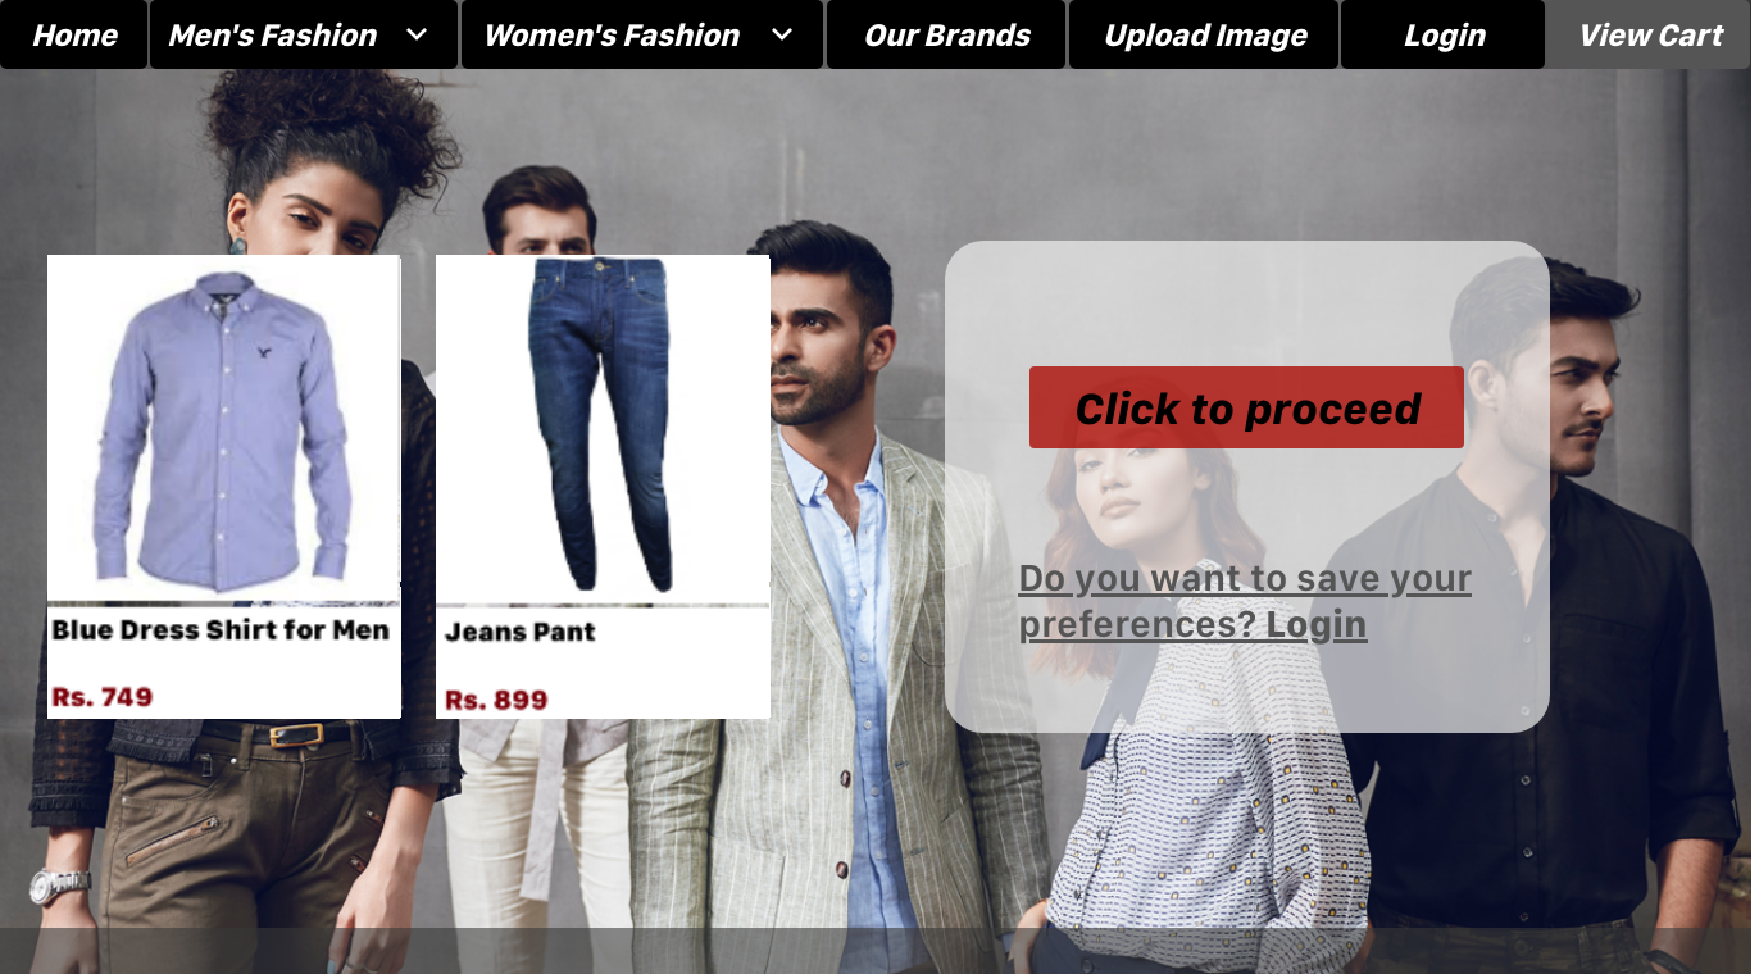
\includegraphics[width=15cm]{images/ViewCart.pdf} 
  \centering
  \caption{View Your Cart Screen}
  \label{gui:cart}
  \end{figure}

  \begin{figure}[H]
  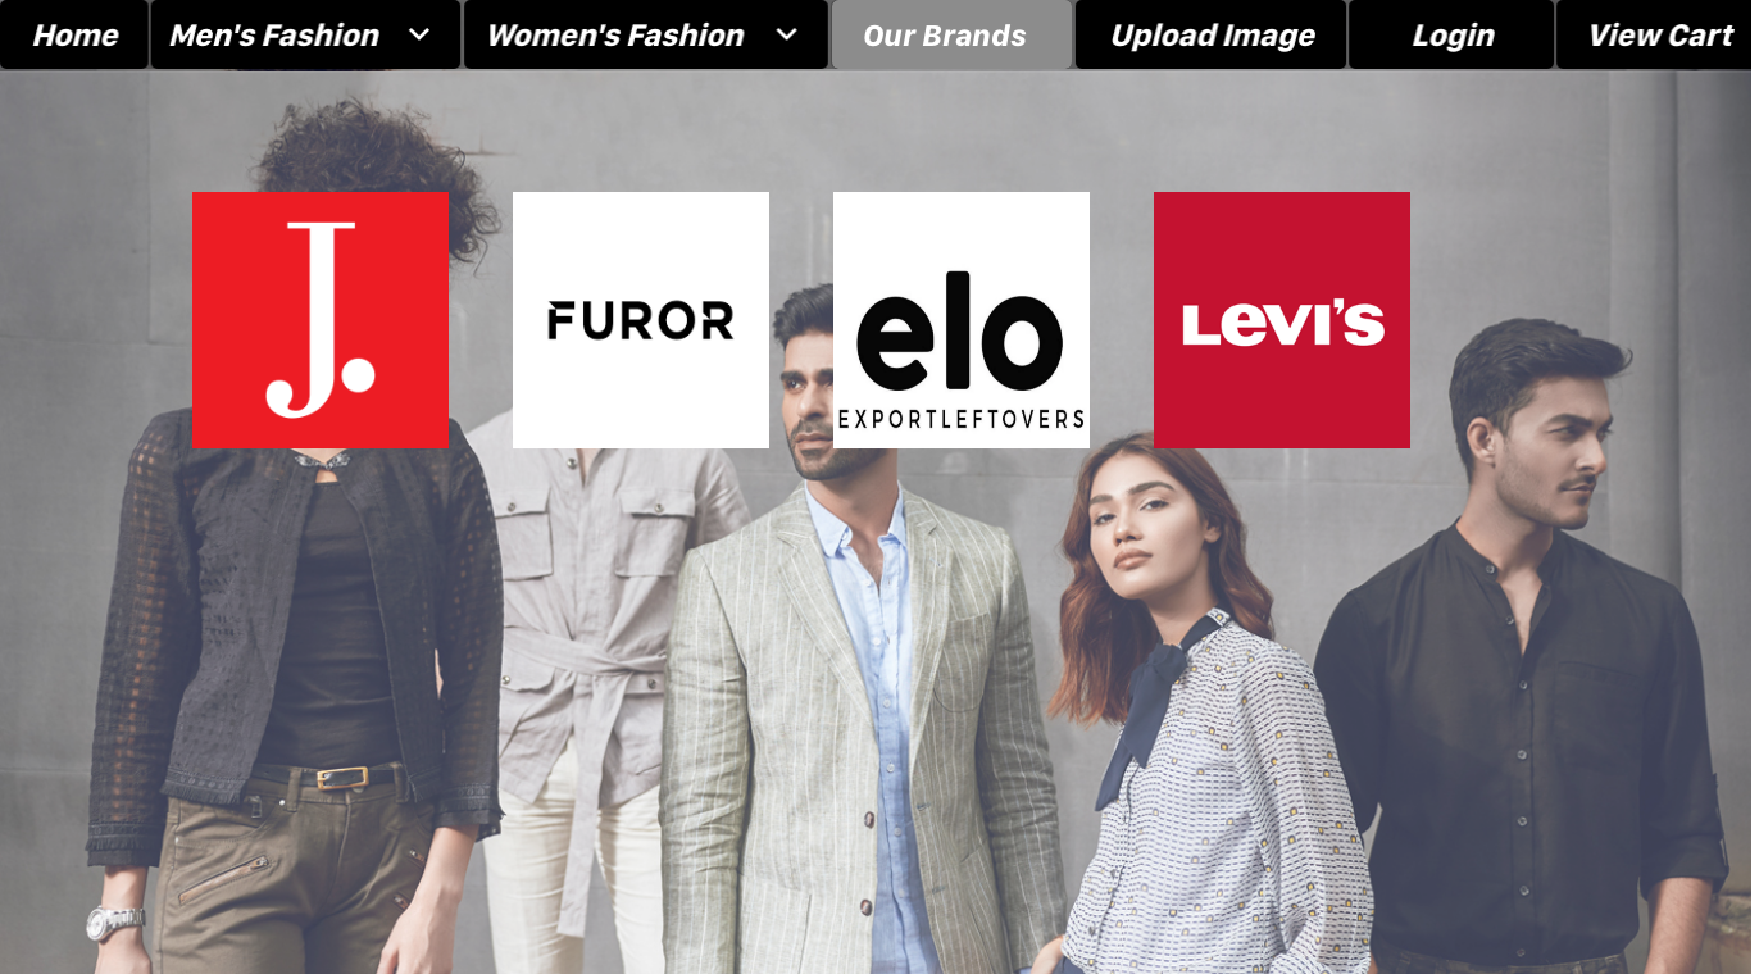
\includegraphics[width=15cm]{images/OurBrands.pdf} 
  \centering
  \caption{Partner Brands Screen}
  \label{gui:brands}
  \end{figure}

   \begin{figure}[H]
  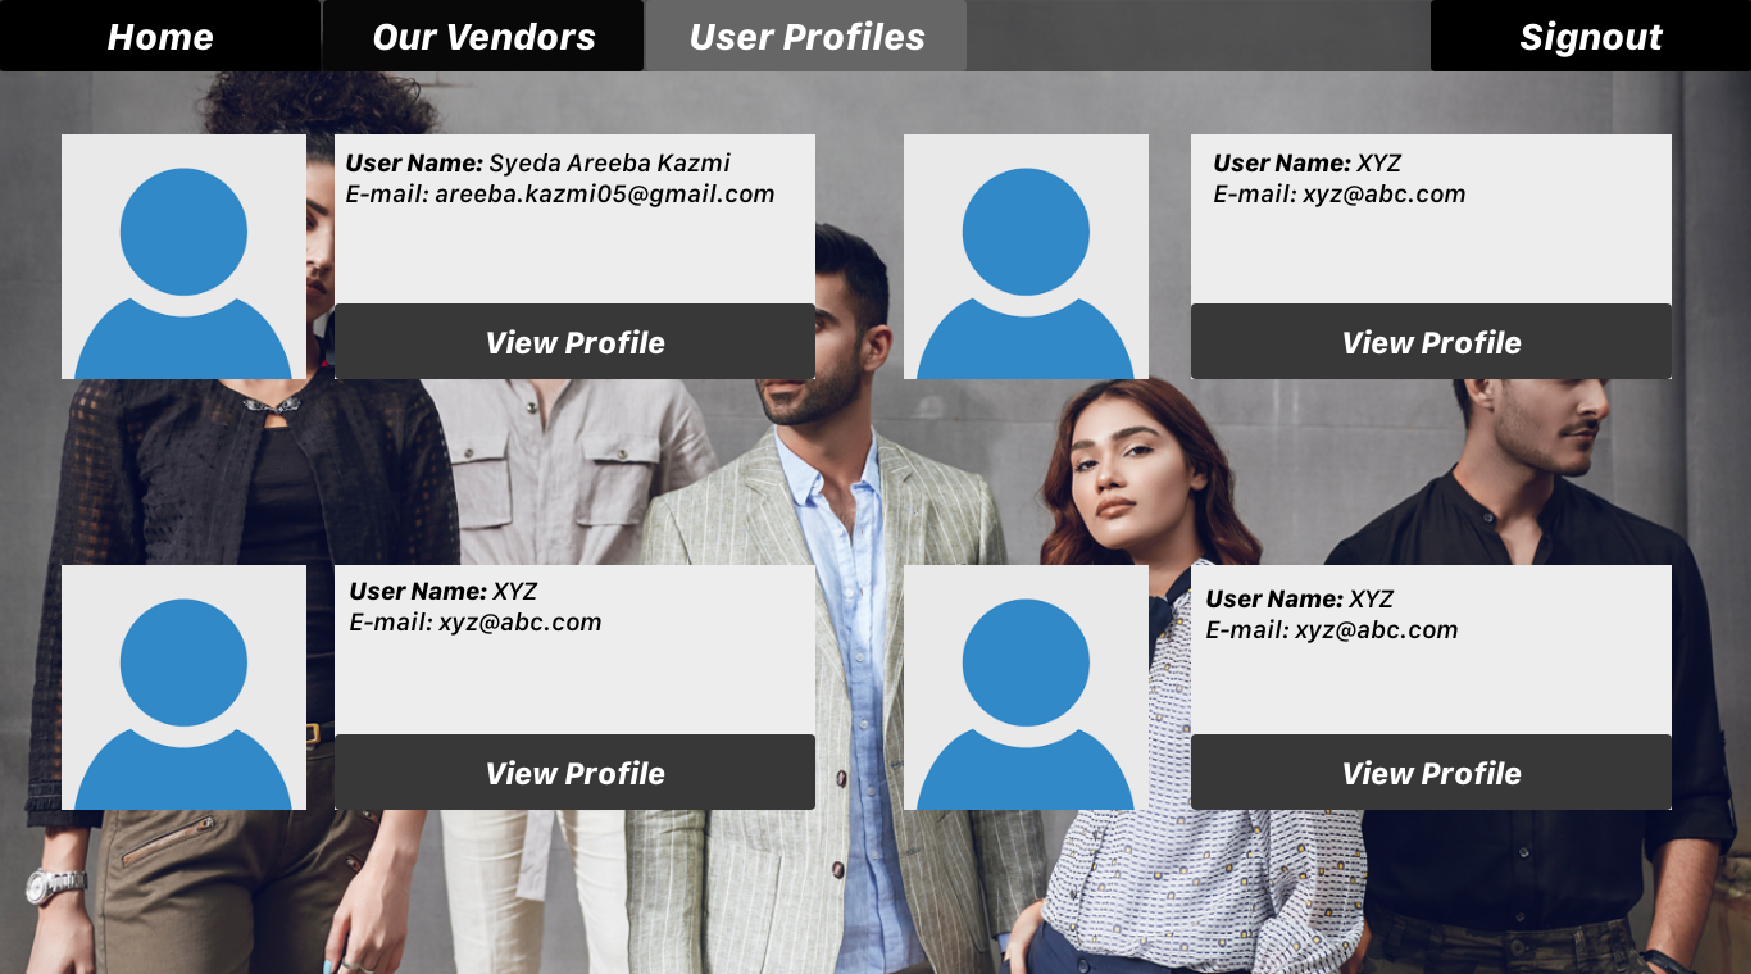
\includegraphics[width=15cm]{images/Profiles1.pdf} 
  \centering
  \caption{Admin-User Profiles Screen 1}
  \label{gui:profiles1}
  \end{figure}

   \begin{figure}[H]
  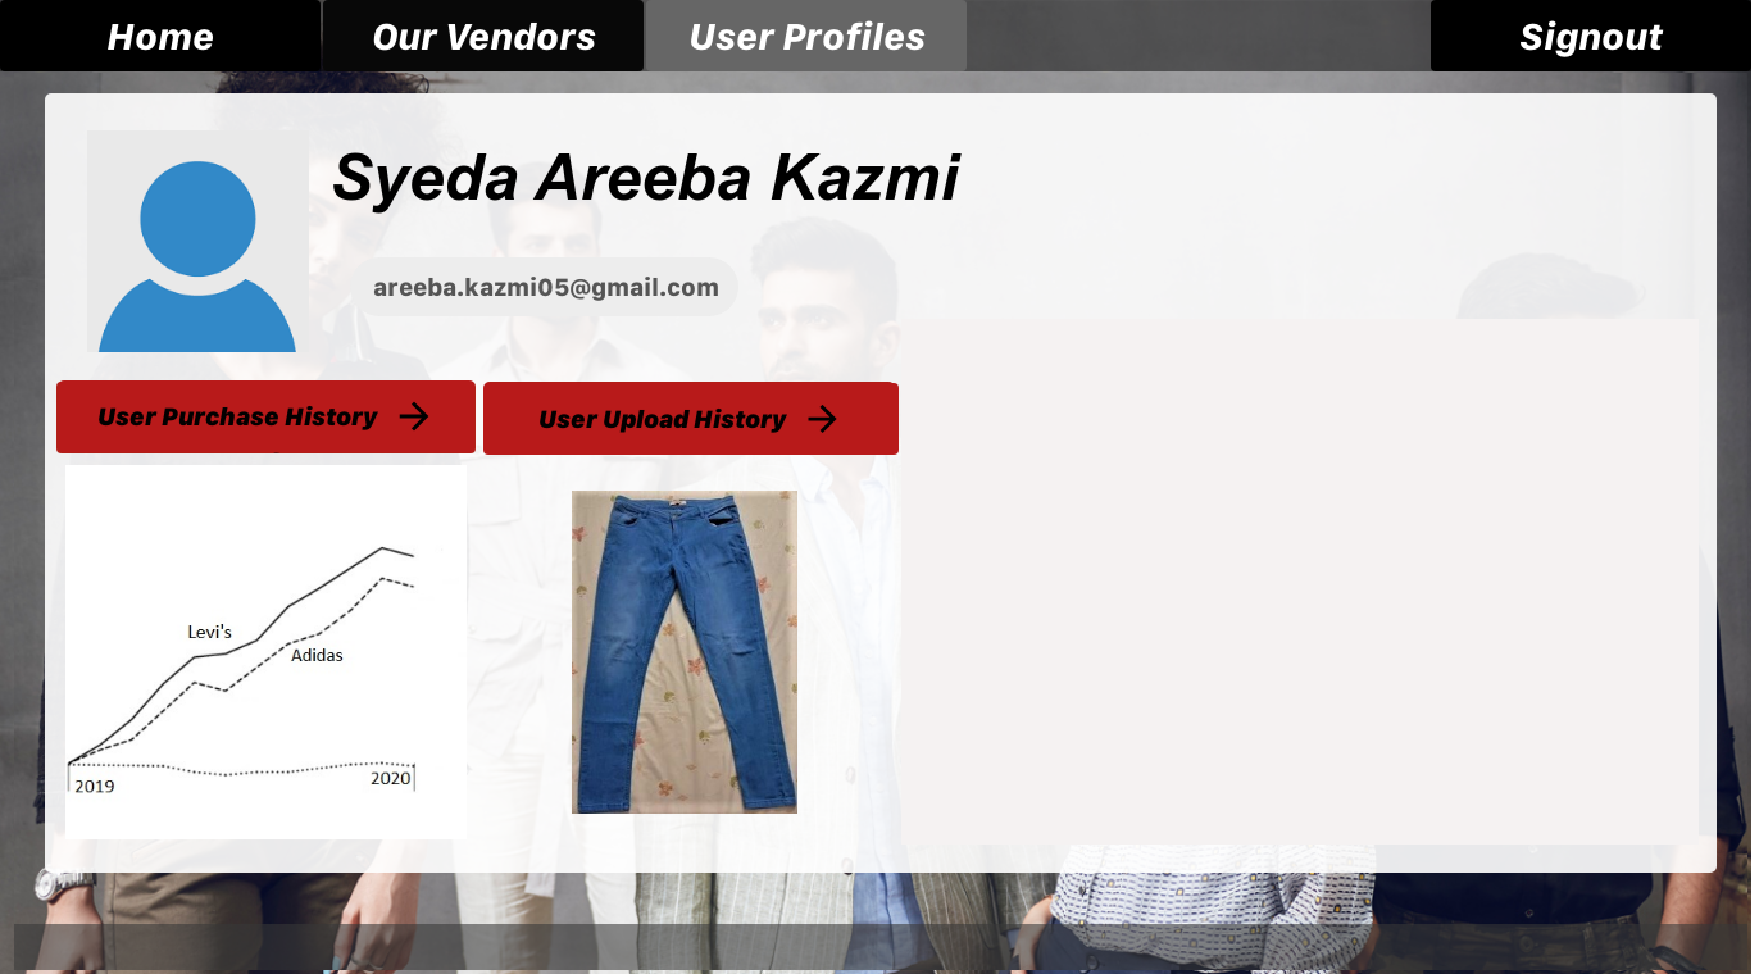
\includegraphics[width=15cm]{images/Profiles2.pdf} 
  \centering
  \caption{Admin-User Profiles Screen 1}
  \label{gui:profiles2}
  \end{figure}

   \begin{figure}[H]
  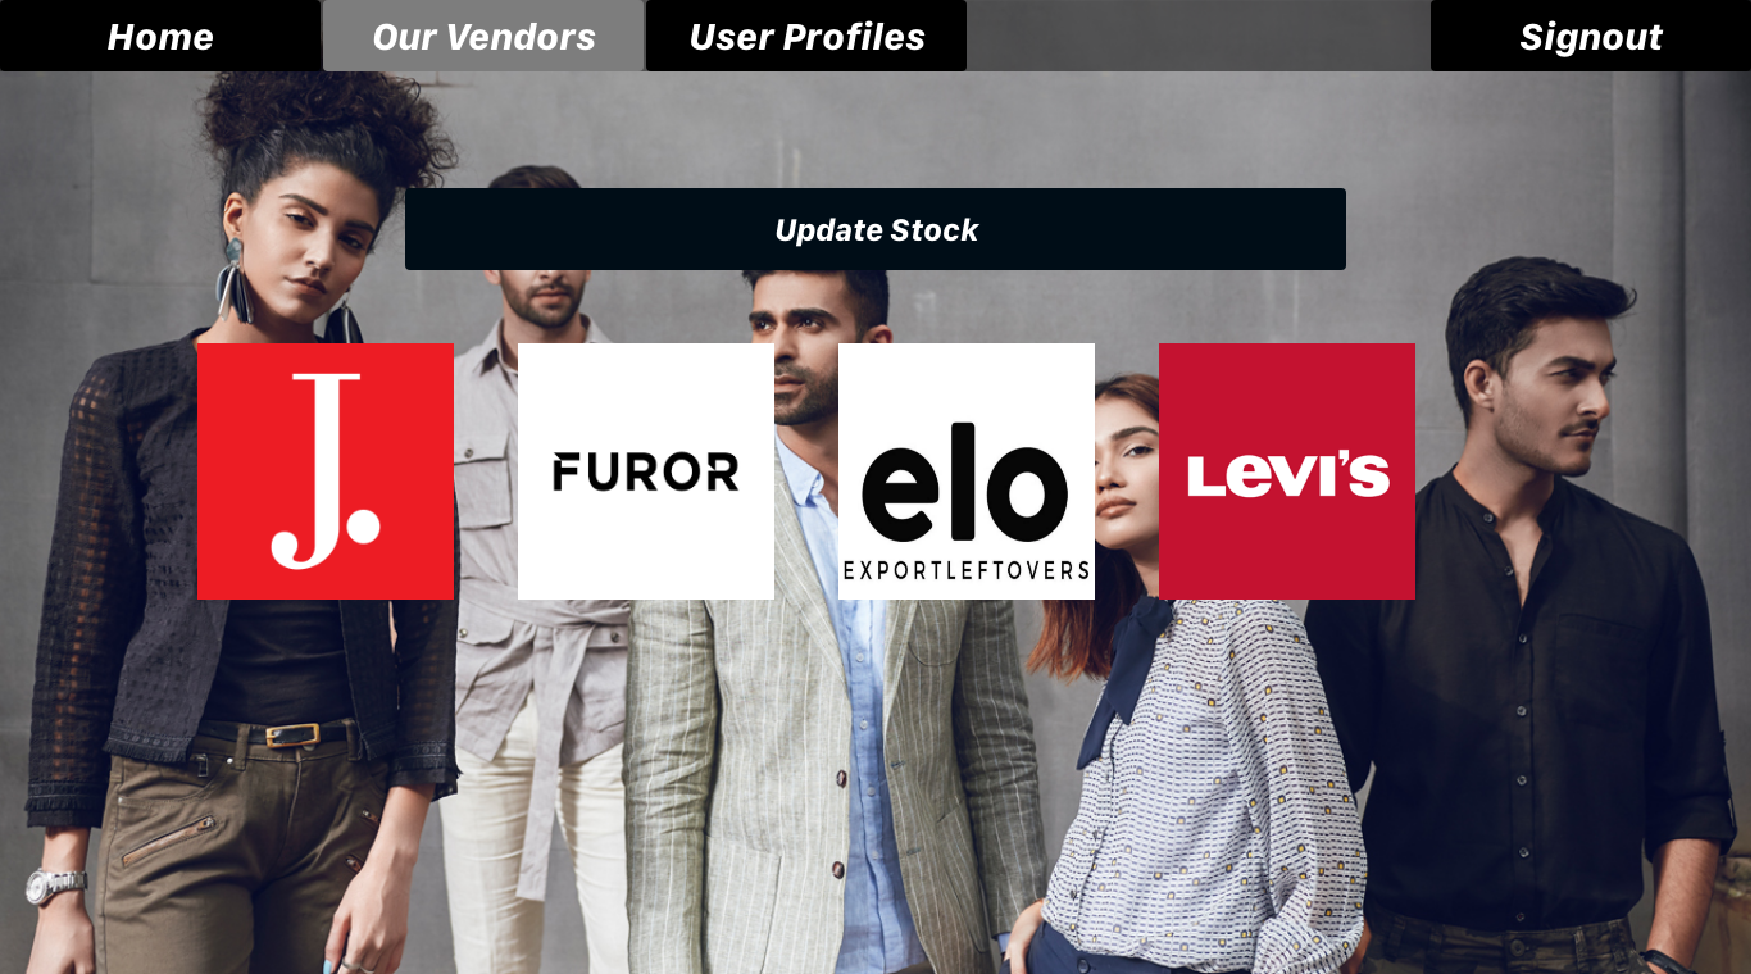
\includegraphics[width=15cm]{images/VendorScreen1.pdf} 
  \centering
  \caption{Admin Vendors Screen 1}
  \label{gui:vendor1}
  \end{figure}

   \begin{figure}[H]
  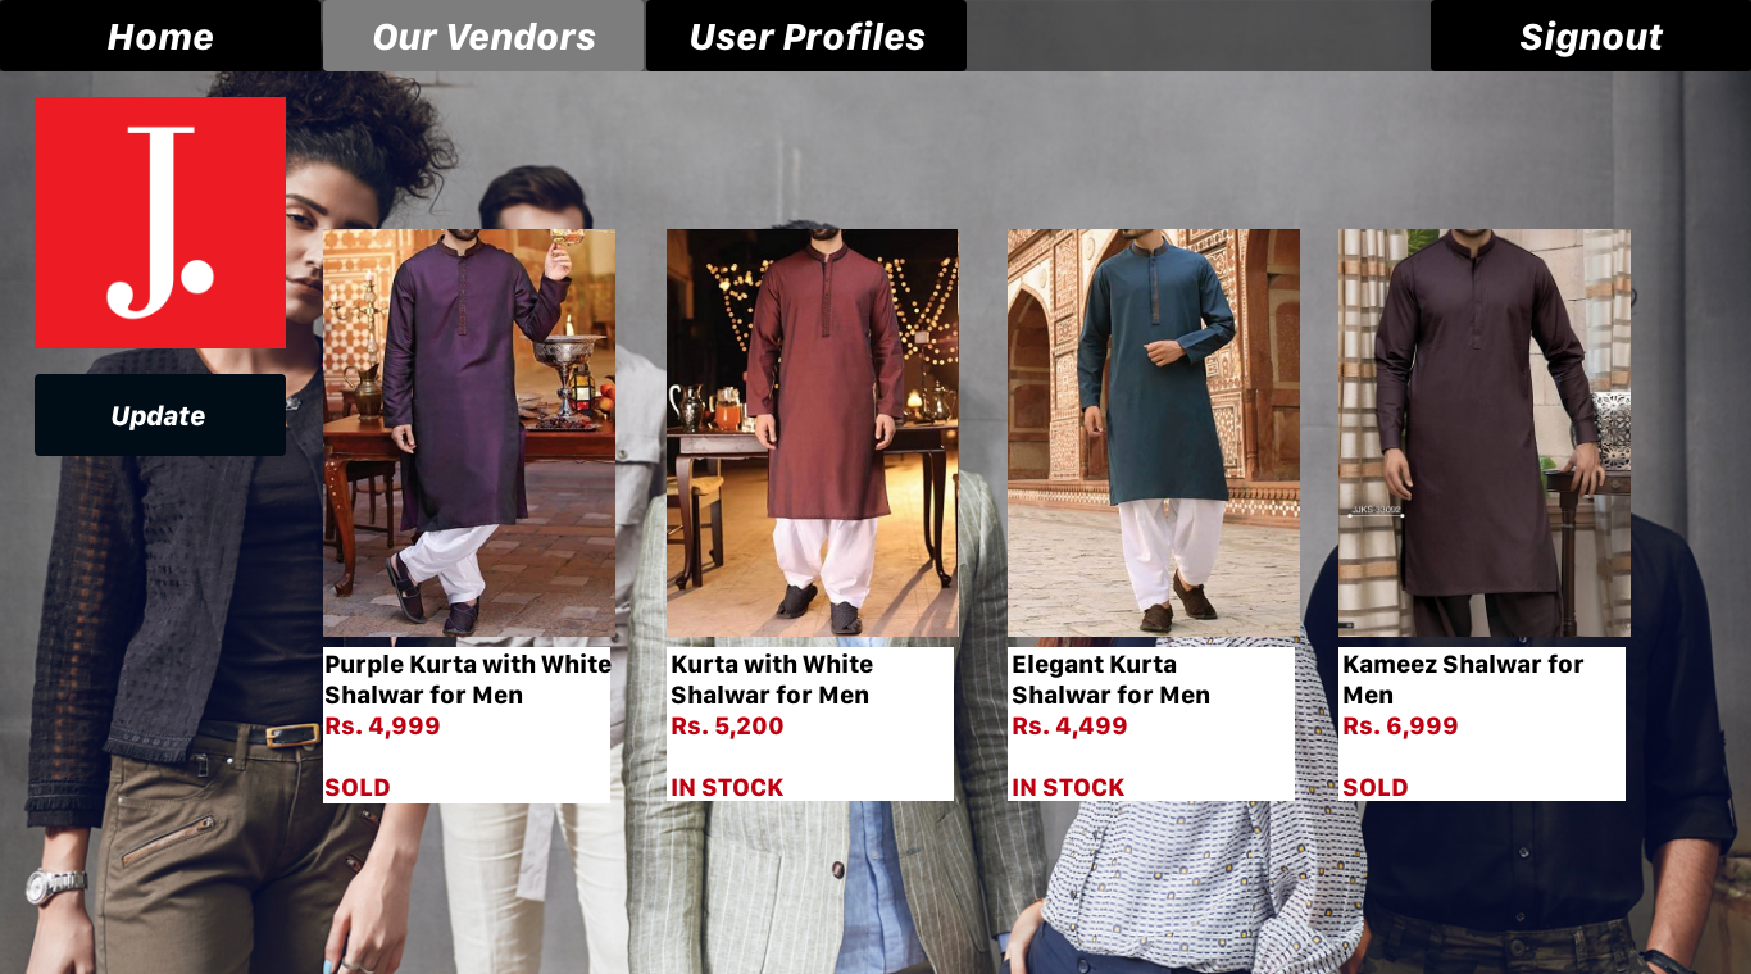
\includegraphics[width=15cm]{images/VendorScreen2.pdf} 
  \centering
  \caption{Admin Vendors Screen 2}
  \label{gui:vendor2}
  \end{figure}

\subsection{Application Program Interface (API)}
The system will be built using the Django framework at the server-end, and React.JS at the client-end (explained in detail in \autoref{srs:sysdiag}). We aim to use REST (Representational State Transfer) APIs, served through the Django REST framework, for all client-server communication since RESTful services as an architectural style would lead to our application being lightweight and scalable. However, since graph-based communication channels are gaining more popularity and adaptation rates in internet technologies these days, and for reasons summarized in \autoref{table:tech-api} ahead, our eventual goal is to establish an API based entirely off of GraphQL. So, for purposes of this web-application, our API will be written primarily as a RESTful service, but will be exposed to the client through a schema-first approach using a GraphQL wrapper. \autoref{api:diag} summarizes this.
\begin{figure}[H]
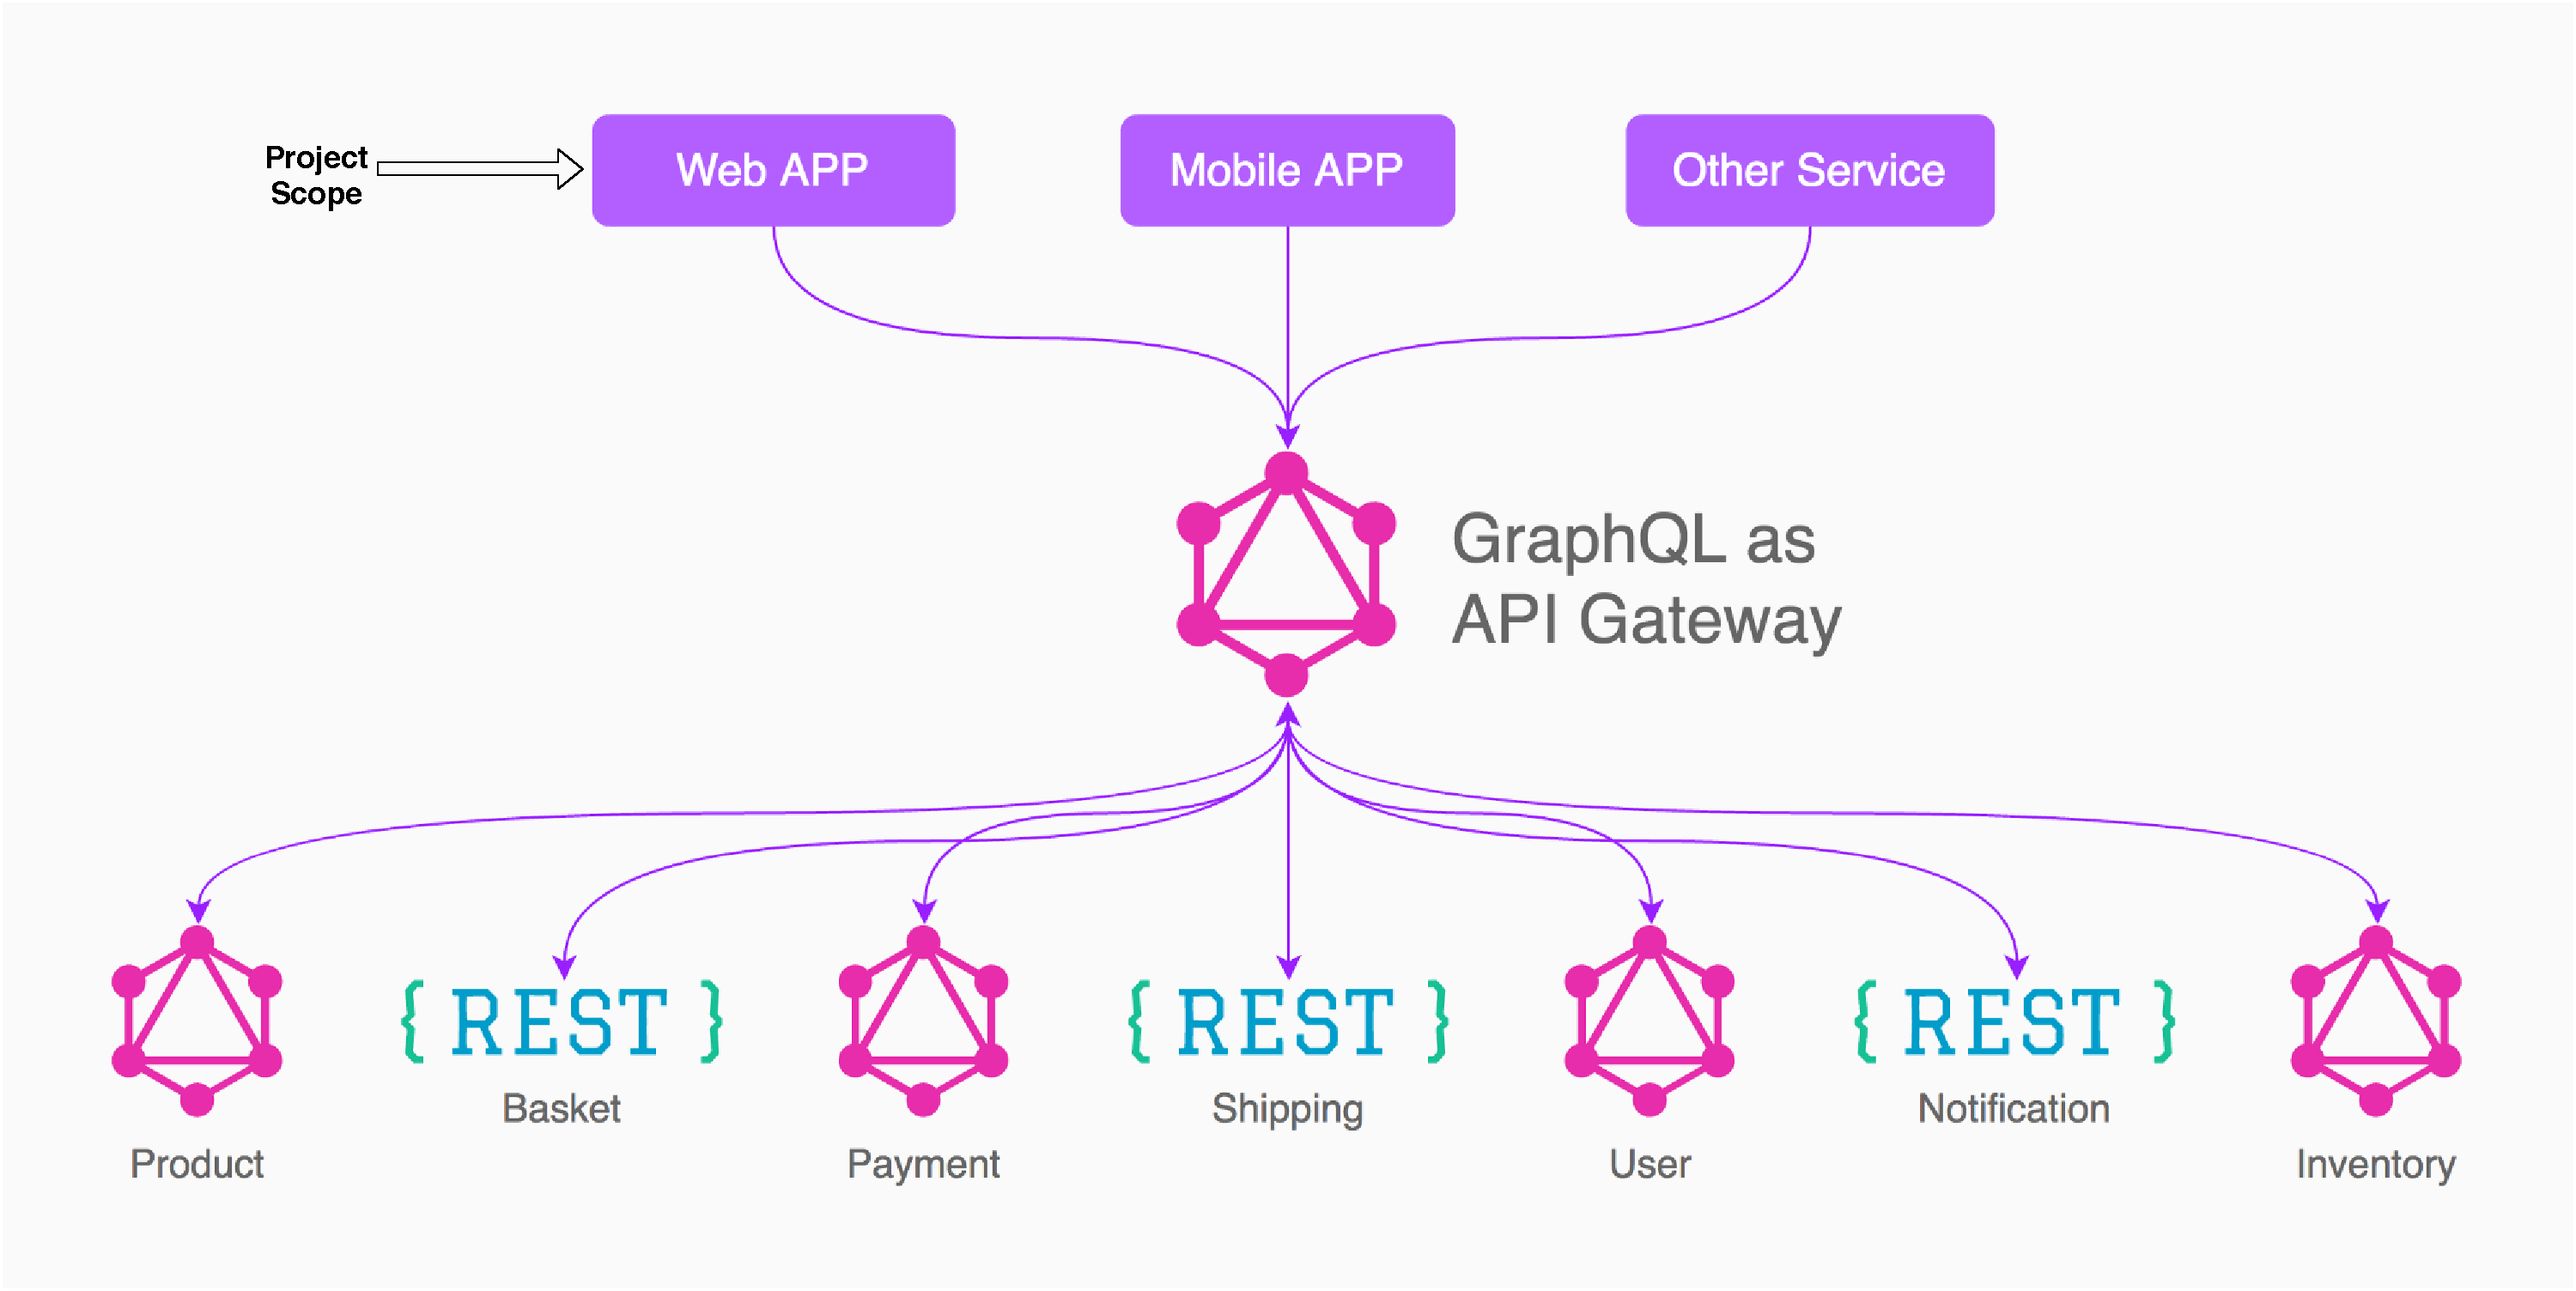
\includegraphics[width=15cm]{images/APIDiagram.pdf} 
\centering
\caption{API Diagram}
\label{api:diag}
\end{figure}

\subsection{Communication Interfaces}
Based on the project requirements and keeping the communication channels in mind, the chosen technology stack for the client-end is: TypeScript, React, and \href{https://github.com/apollographql/react-apollo}{React Apollo} (for interacting with the GraphQL API), and for the server-end is: Python, Django, and \href{https://github.com/graphql-python/graphene-django}{Graphene Django} (for creating the GraphQL API). \autoref{table:tech-server}, \autoref{table:tech-client}, and \autoref{table:tech-api} offer a detailed comparison between why these communication interfaces were picked over some of their major competitors.


\section{Use Cases}
The two main users of the system are customers and the admin. \autoref{usecases} summarizes their system use cases.
\begin{figure}[H]
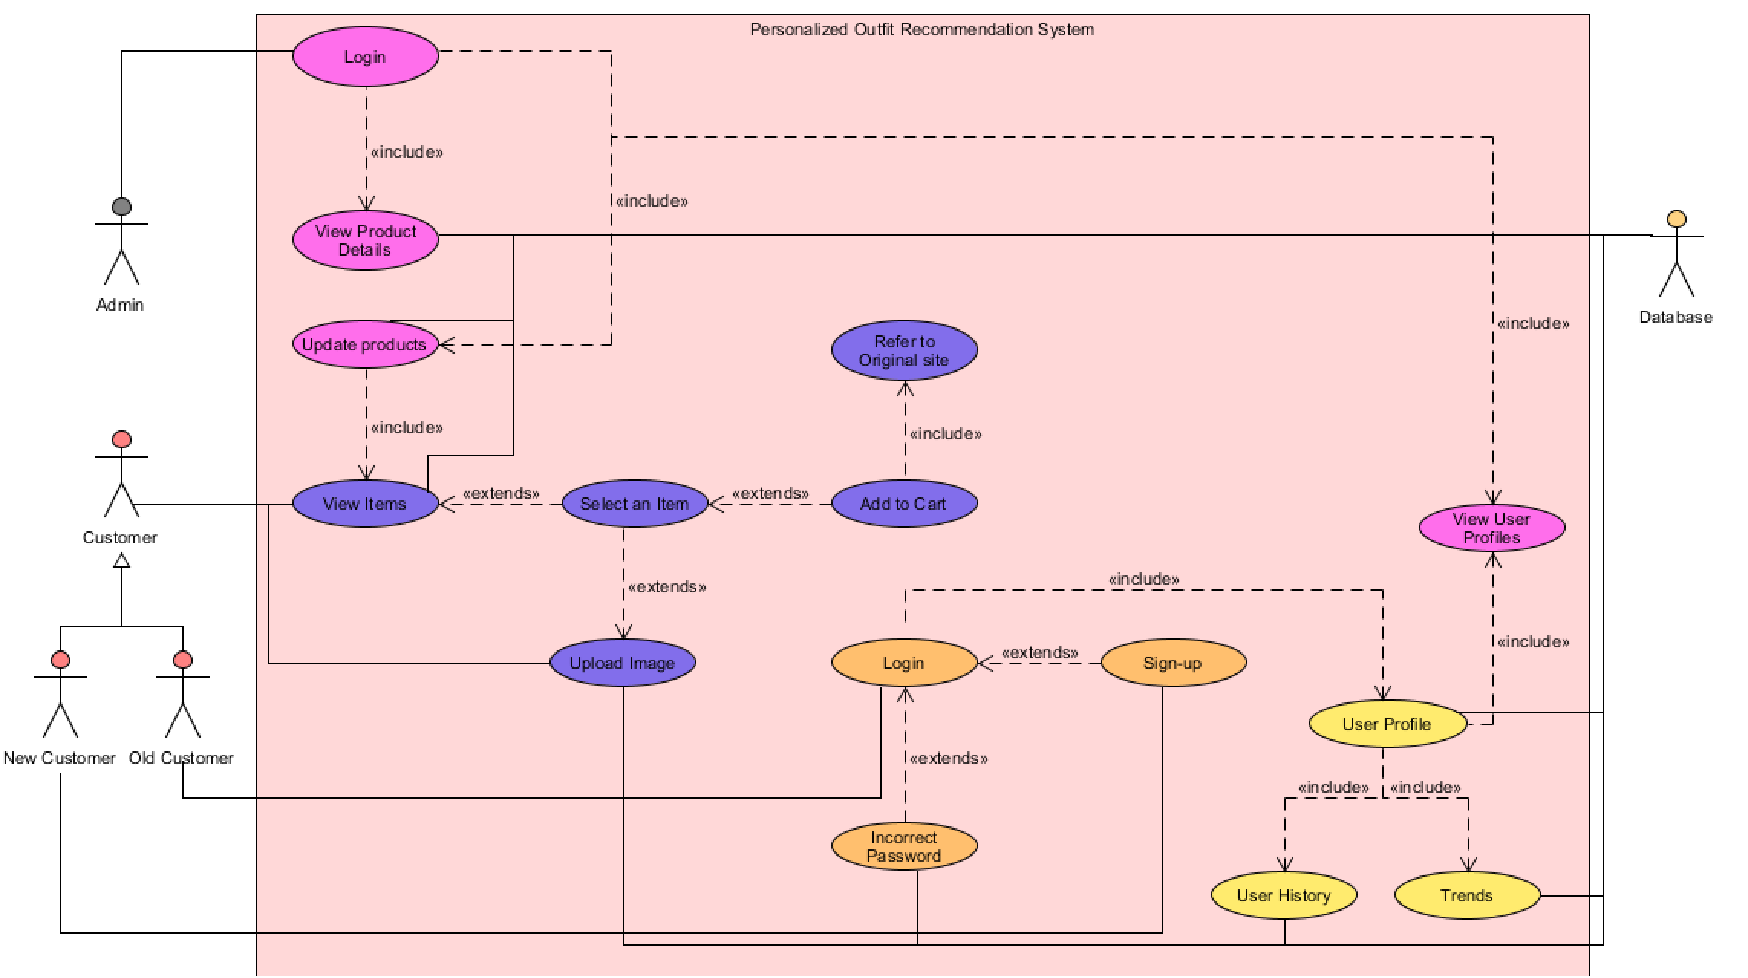
\includegraphics[width=15cm]{images/UseCaseDiag.pdf} 
\centering
\caption{Use-Case Diagram}
\label{usecases}
\end{figure}


\subsection{User Login}
\begin{center}
    \begin{tabular}{ @{}|p{7cm}||p{7cm}|  }
    \hline
    Use-Case Name: & Login  \\ \hline
    Use-Case ID: & PORS-01 \\ \hline
    Priority: & High \\ \hline
    Primary Business Actor: & System Admin \\ \hline
    Other Participating Actors: & Customer \\ \hline
    Description: & System admin needs to login in order to view customer, product details and update the stock. Whereas, the customer needs to login to view the referred sites and save his profile \\ \hline
    Pre-condition: & User has registered previously on the app and has valid email and password.  \\ \hline
    Trigger: & This use case is initiated when the admin wants to navigate the app or customer tries to view the referred site. \\ \hline
    Typical course of events: & \textbf{Actor Action:} \newline Actor enters valid username and password. \newline \textbf{System Action:} \newline Checks if the given username is registered in database and the given password is valid.
 \\ \hline
    Alternate courses: & If the credentials are invalid then an error message is displayed.  \\ \hline
    Conclusion: &  User successfully logs in using valid credentials.\\ \hline
    Post-condition: & User login is logged in the database. \\ \hline
    \end{tabular}
\end{center}

\subsection{View Product Details}
\begin{center}
    \begin{tabular}{ @{}|p{7cm}||p{7cm}|  }
    \hline
    Use-Case Name: & View Product Details  \\ \hline
    Use-Case ID: & PORS-02 \\ \hline
    Priority: & High \\ \hline
    Primary Business Actor: & System Admin \\ \hline
    Other Participating Actors: & Customer \\ \hline
    Description: & System Admin will view the product details to be able to update the stock. Whereas the customer will be able to see the product with details in order to select the items of their choice. \\ \hline
    Pre-condition: & Logged in as Admin or Customer.  \\ \hline
    Trigger: & This use case is triggered when the user clicks a product. \\ \hline
    Typical course of events: & Appropriate product details will be displayed to the user. \\ \hline
    Alternate courses: & None \\ \hline
    Conclusion: &  The user is able to see the product detail page.\\ \hline
    Post-condition: & User search is logged in the database.  \\ \hline
    \end{tabular}
\end{center}

\subsection{Update Stock}

\begin{center}
    \begin{tabular}{ @{}|p{7cm}||p{7cm}|  }
    \hline
    Use-Case Name: & Update Stock  \\ \hline
    Use-Case ID: & PORS-03 \\ \hline
    Priority: & High \\ \hline
    Primary Business Actor: & System Admin \\ \hline
    Other Participating Actors: & None \\ \hline
    Description: & System Admin will be able to update new stock and product details in case a product is sold out. \\ \hline
    Pre-condition: & Logged in as Admin.  \\ \hline
    Trigger: & This use case will be triggered when the system admin clicks update stock button. \\ \hline
    Typical course of events: & \textbf{System Action:} \newline System will check all the products and update the sold out and new products accordingly.
 \\ \hline
    Alternate courses: & None \\ \hline
    Conclusion: & The stock is successfully updated. \\ \hline
    Post-condition: & Customers are able to view the updated stock.\\ \hline
    \end{tabular}
\end{center}

\subsection{Upload an Image}

\begin{center}
    \begin{tabular}{ @{}|p{7cm}||p{7cm}|  }
    \hline
    Use-Case Name: & Upload an Image  \\ \hline
    Use-Case ID: & PORS-04 \\ \hline
    Priority: & High \\ \hline
    Primary Business Actor: & Customer \\ \hline
    Other Participating Actors: & None \\ \hline
    Description: & Application will allow customers to upload an image of their piece of clothing in order to find a similar or complementary items. \\ \hline
    Pre-condition: & None \\ \hline
    Trigger: & This use case will be triggered when the user will click upload image option. \\ \hline
    Typical course of events: & \textbf{System Action:} \newline System will check if the uploaded photo is of a piece of clothing
 \\ \hline
    Alternate courses: & If the uploaded image is not recognizable, a suitable error message is displayed. \\ \hline
    Conclusion: & Customer’s valid picture will be uploaded on the app. \\ \hline
    Post-condition: & Customer will be able to see the recommendation according to the uploaded picture. \\ \hline
    \end{tabular}
\end{center}

\subsection{Add to Cart}

\begin{center}
    \begin{tabular}{ @{}|p{7cm}||p{7cm}|  }
    \hline
    Use-Case Name: & Add to Cart  \\ \hline
    Use-Case ID: & PORS-05 \\ \hline
    Priority: & High \\ \hline
    Primary Business Actor: & Customer \\ \hline
    Other Participating Actors: & None \\ \hline
    Description: & Items selected by the customer will be added to the cart in order to proceed to the original referral site. \\ \hline
    Pre-condition: & None \\ \hline
    Trigger: & This use case will be triggered when the customer will select an item and click the option ‘add to cart’. \\ \hline
    Typical course of events: & System will check if the product is available to be added to the cart. \\ \hline
    Alternate courses: & None \\ \hline
    Conclusion: &  Selected item will be added to the customer’s cart.\\ \hline
    Post-condition: &  Valid referral link to the item is updated. \\ \hline
    \end{tabular}
\end{center}

\subsection{Refer to Original Sites}
\begin{center}
    \begin{tabular}{ @{}|p{7cm}||p{7cm}|  }
    \hline
    Use-Case Name: & Refer to Original Sites  \\ \hline
    Use-Case ID: & PORS-06 \\ \hline
    Priority: & Medium \\ \hline
    Primary Business Actor: & Customer \\ \hline
    Other Participating Actors: & None \\ \hline
    Description: & Once the customer has selected items of his choice, those will be added to the cart and then he would be redirected to the original product site.
 \\ \hline
    Pre-condition: & Items added to the cart \\ \hline
    Trigger: & This use case will be triggered when a customer clicks on ‘proceed to original site’ option, available in his cart. \\ \hline
    Typical course of events: & \textbf{System Action:} \newline System will direct the customer to the original sites of the items available in customer’s cart
 \\ \hline
    Alternate courses: & None\\ \hline
    Conclusion: &  Customer directed to the original sites of the items he has chosen.\\ \hline
    Post-condition: &  Reference point is logged in the dataset. \\ \hline
    \end{tabular}
\end{center}

\subsection{Sign-up}

\begin{center}
    \begin{tabular}{ @{}|p{7cm}||p{7cm}|  }
    \hline
    Use-Case Name: & Sign-up  \\ \hline
    Use-Case ID: & PORS-07 \\ \hline
    Priority: & High \\ \hline
    Primary Business Actor: & Admin \\ \hline
    Other Participating Actors: & Customer \\ \hline
    Description: & Admin and Customers will have to sign-up and register on the app in order to login and proceed. \\ \hline
    Pre-condition: & Valid information by the user. \\ \hline
    Trigger: & This use case will be triggered when a new user wants to register on the application. \\ \hline
    Typical course of events: & \textbf{Actor Action:} \newline Providing valid details.\newline \textbf{System Action:} \newline Checking if the details provided are available in the database.
 \\ \hline
    Alternate courses: & If the details provided are incomplete or already registered then appropriate error message must be displayed. \\ \hline
    Conclusion: &  User is able to sign-up successfully.\\ \hline
    Post-condition: & New user is added to the database. \\ \hline
    \end{tabular}
\end{center}

\subsection{Incorrect Password}
\begin{center}
    \begin{tabular}{ @{}|p{7cm}||p{7cm}|  }
    \hline
    Use-Case Name: & Incorrect Password \\ \hline
    Use-Case ID: & PORS-08\\ \hline
    Priority: & High \\ \hline
    Primary Business Actor: & Admin, Customer \\ \hline
    Other Participating Actors: &  None \\ \hline
    Description: & While logging-in on the app, the user must enter a valid email and password.\\ \hline
    Pre-condition: & Registered on the app. \\ \hline
    Trigger: &  This use case will be triggered when a user tried to login with incorrect password or username. \\ \hline
    Typical course of events: & \textbf{System Action:} \newline System checks if the given password or user-name is registered in the database.  \\ \hline
    Alternate courses: & System displays an error message about incorrect credentials. \\ \hline
    Conclusion: & User unable to login to the app. \\ \hline
    Post-condition: & Incorrect login attempt is logged in the database. \\ \hline
    \end{tabular}
\end{center}

\subsection{User Profile}
\begin{center}
    \begin{tabular}{ @{}|p{7cm}||p{7cm}|  }
    \hline
    Use-Case Name: & User Profile \\ \hline
    Use-Case ID: & PORS-09 \\ \hline
    Priority: & Medium \\ \hline
    Primary Business Actor: & Customer \\ \hline
    Other Participating Actors: & System Admin \\ \hline
    Description: & All registered users will have user profiles displaying their details, purchase history and uploaded image history. \\ \hline
    Pre-condition: & User must be logged in. \\ \hline
    Trigger: & This use case will be triggered when the admin wants to look at a particular user’s profile or the customer himself clicks at his profile. \\ \hline
    Typical course of events: &  System will display the updated user profile to the user. \\ \hline
    Alternate courses: & None \\ \hline
    Conclusion: &  User profile displayed.\\ \hline
    Post-condition: &  None\\ \hline
    \end{tabular}
\end{center}

\subsection{User History}
\begin{center}
    \begin{tabular}{ @{}|p{7cm}||p{7cm}|  }
    \hline
    Use-Case Name: & User History \\ \hline
    Use-Case ID: & PORS-10\\ \hline
    Priority: & Medium \\ \hline
    Primary Business Actor: & Customer \\ \hline
    Other Participating Actors: & System Admin \\ \hline
    Description: & All registered users will have their user history comprising of purchase history and uploaded image history. \\ \hline
    Pre-condition: & 1.	User is registered in the database. \newline 2. User has either purchased or uploaded an image before.
 \\ \hline
    Trigger: & This use case will be triggered when a user purchases an item or uploads any image. \\ \hline
    Typical course of events: &  System will update the user history when the user will purchase or upload an item.\\ \hline
    Alternate courses: & None\\ \hline
    Conclusion: & User history is updated at every purchase or upload, given that the user is logged in.\\ \hline
    Post-condition: &  None\\ \hline
    \end{tabular}
\end{center}

\subsection{View Trends}
\begin{center}
    \begin{tabular}{ @{}|p{7cm}||p{7cm}|  }
    \hline
    Use-Case Name: & View Trends \\ \hline
    Use-Case ID: & PORS-11 \\ \hline
    Priority: & Medium \\ \hline
    Primary Business Actor: & Customer \\ \hline
    Other Participating Actors: & None \\ \hline
    Description: & Different statistics will be displayed indicating the sales or ratings of each brand in last 30 days.  \\ \hline
    Pre-condition: &  users have either purchased or rated an item from any brand.\\ \hline
    Trigger: &  This use case will be triggered when the user clicks trend option. \\ \hline
    Typical course of events: & System will update the trend at each purchase or rating by the user. \\ \hline
    Alternate courses: & None\\ \hline
    Conclusion: &  User is able to see the most updated trends. \\ \hline
    Post-condition: &  Catalog matrix is updated in the database.\\ \hline
    \end{tabular}
\end{center}

\section{Datasets}
This section describes the specific dataset which will be used to build our system. An appropriate snapshot of the dataset is also included in . Futher details, whenever needed, will be presented in the appendix.

For purposes of the image classification pipeline for our recommendation engine, we have selected DeepFashion \cite{DeepFashion} as our preliminary dataset. The dataset consists over 800,000 diverse fashion images ranging from well-posed shop images to unconstrained consumer photos. What makes this dataset suitable towards our system is the fact that it is annotated with rich information of clothing items. Each image in this dataset is labelled with 50 categories, 1,000 descriptive attributes, bounding box and clothing landmarks, and this would kick-start the training of our classifier. A category-wise subset of the dataset is depicted in \autoref{dataset:DeepFashion}. 

It is important to clarify here that the DeepFashion dataset consists of product images from western stores and outlets, so the classifier would not generalize efficiently to products in the local eastern domain, which is a  requirement of our system. Moreover, there are limitations in the amount of products and datasets we can scrape from eastern fashion stores such as J., Export Leftovers, Zellbury, Daraz, etc. If we were to use these as the only data for training our classifier, the model would indubitably suffer from underfitting. In order to maintain a good fit, we will use the concept of Transfer Learning to re-train the classifier trained on DeepFashion on our local scraped dataset from the aforementioned local fashion stores.

\begin{figure}[H]
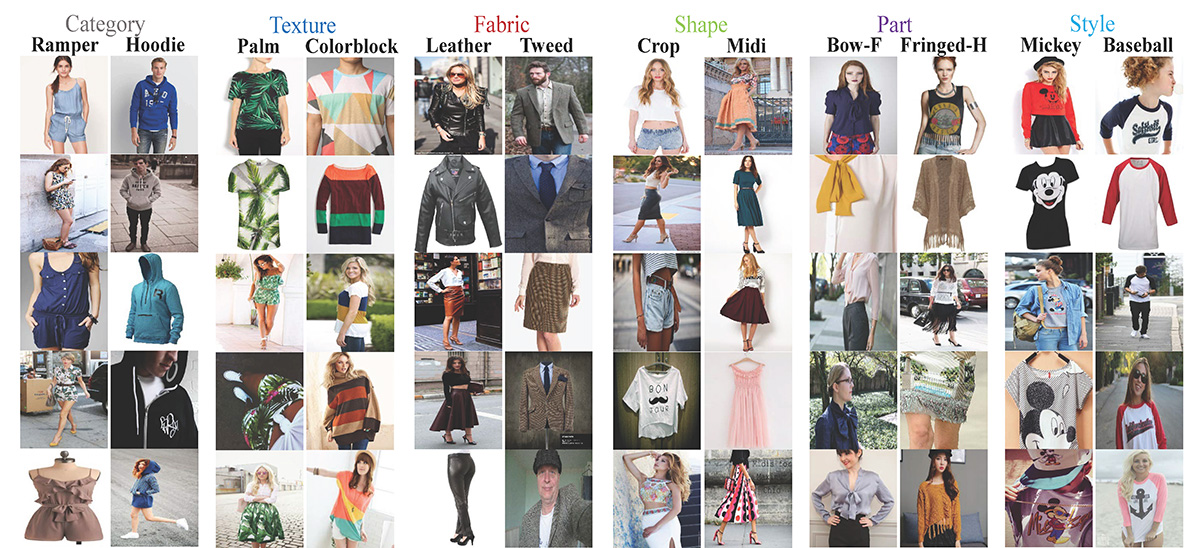
\includegraphics[width=15cm]{images/DeepFashion.pdf} 
\centering
\caption{The DeepFashion Dataset}
\label{dataset:DeepFashion}
\end{figure}

\section{System Diagram}
\label{srs:sysdiag}
\autoref{sysdiag:module} gives an overview of different modules of our system.
\begin{figure}[H]
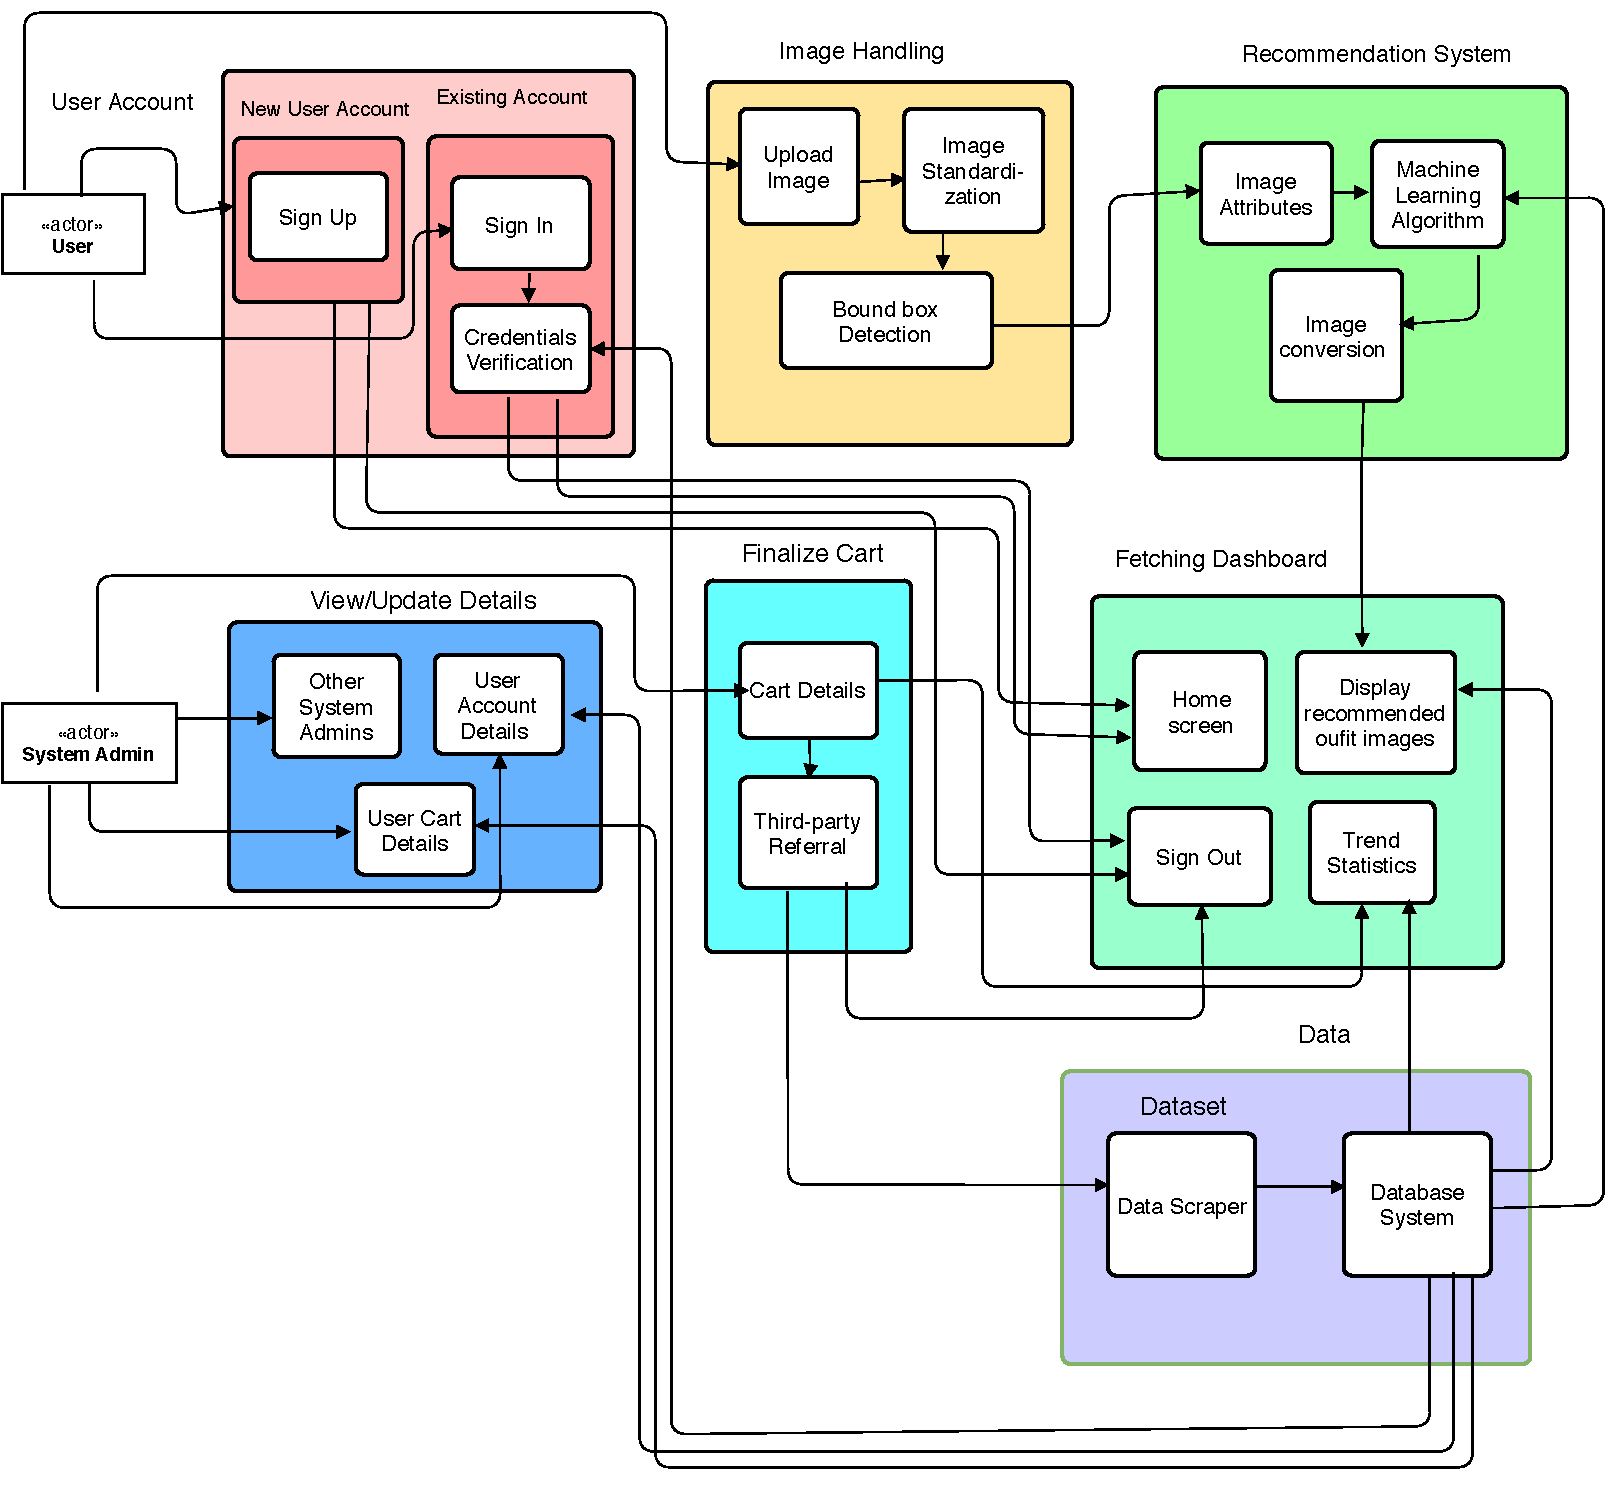
\includegraphics[width=15cm]{images/systemDiagramModule.pdf} 
\centering
\caption{Module-wise System Diagram}
\label{sysdiag:module}
\end{figure}
\autoref{sysdiag:tech} gives an overview of the chosen architecture of our system.
\begin{figure}[H]
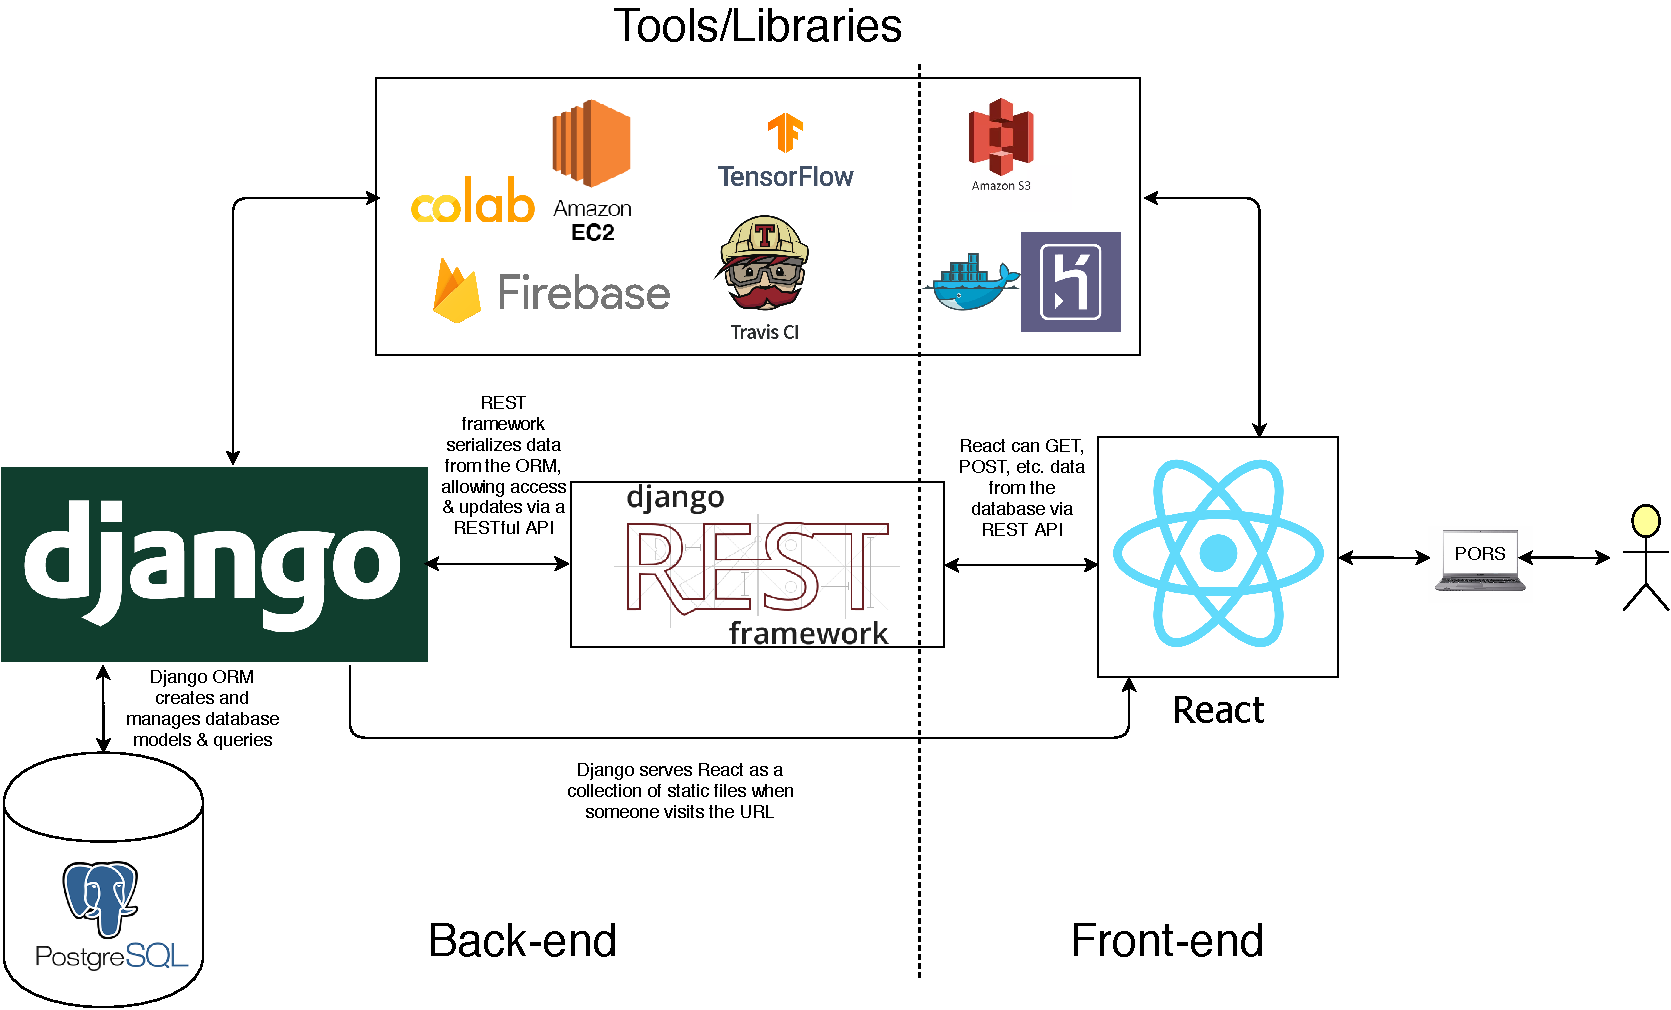
\includegraphics[width=15cm]{images/systemDiagramTech.pdf} 
\centering
\caption{Technology-wise System Diagram}
\label{sysdiag:tech}
\end{figure}

\section{Data Flow Diagram}
Rudimentary data flow diagrams for the system have also been constructed, given below in \autoref{dfd:context} and \autoref{dfd:zero}:

\begin{figure}[H]
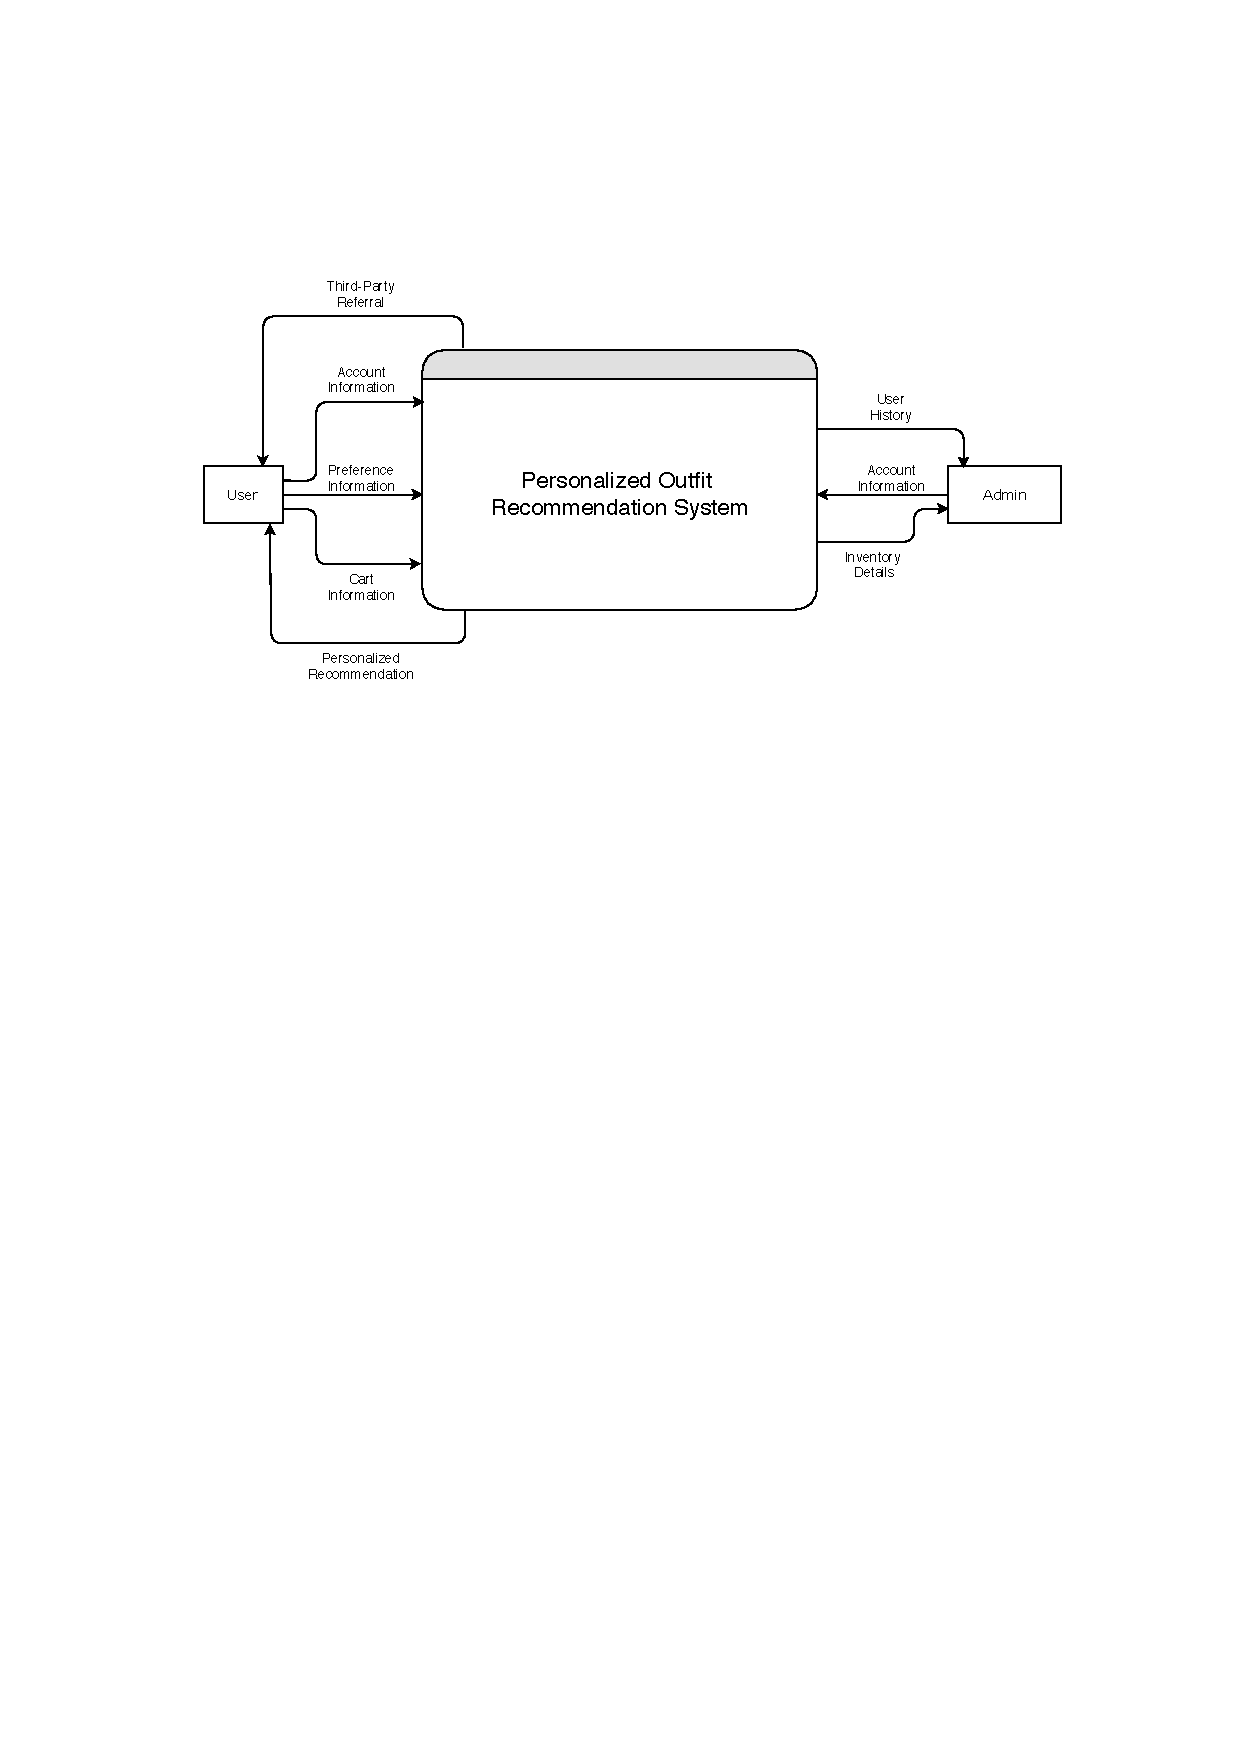
\includegraphics[width=15cm]{images/dfdContext.pdf} 
\centering
\caption{Context Level DFD}
\label{dfd:context}
\end{figure}

\begin{figure}[H]
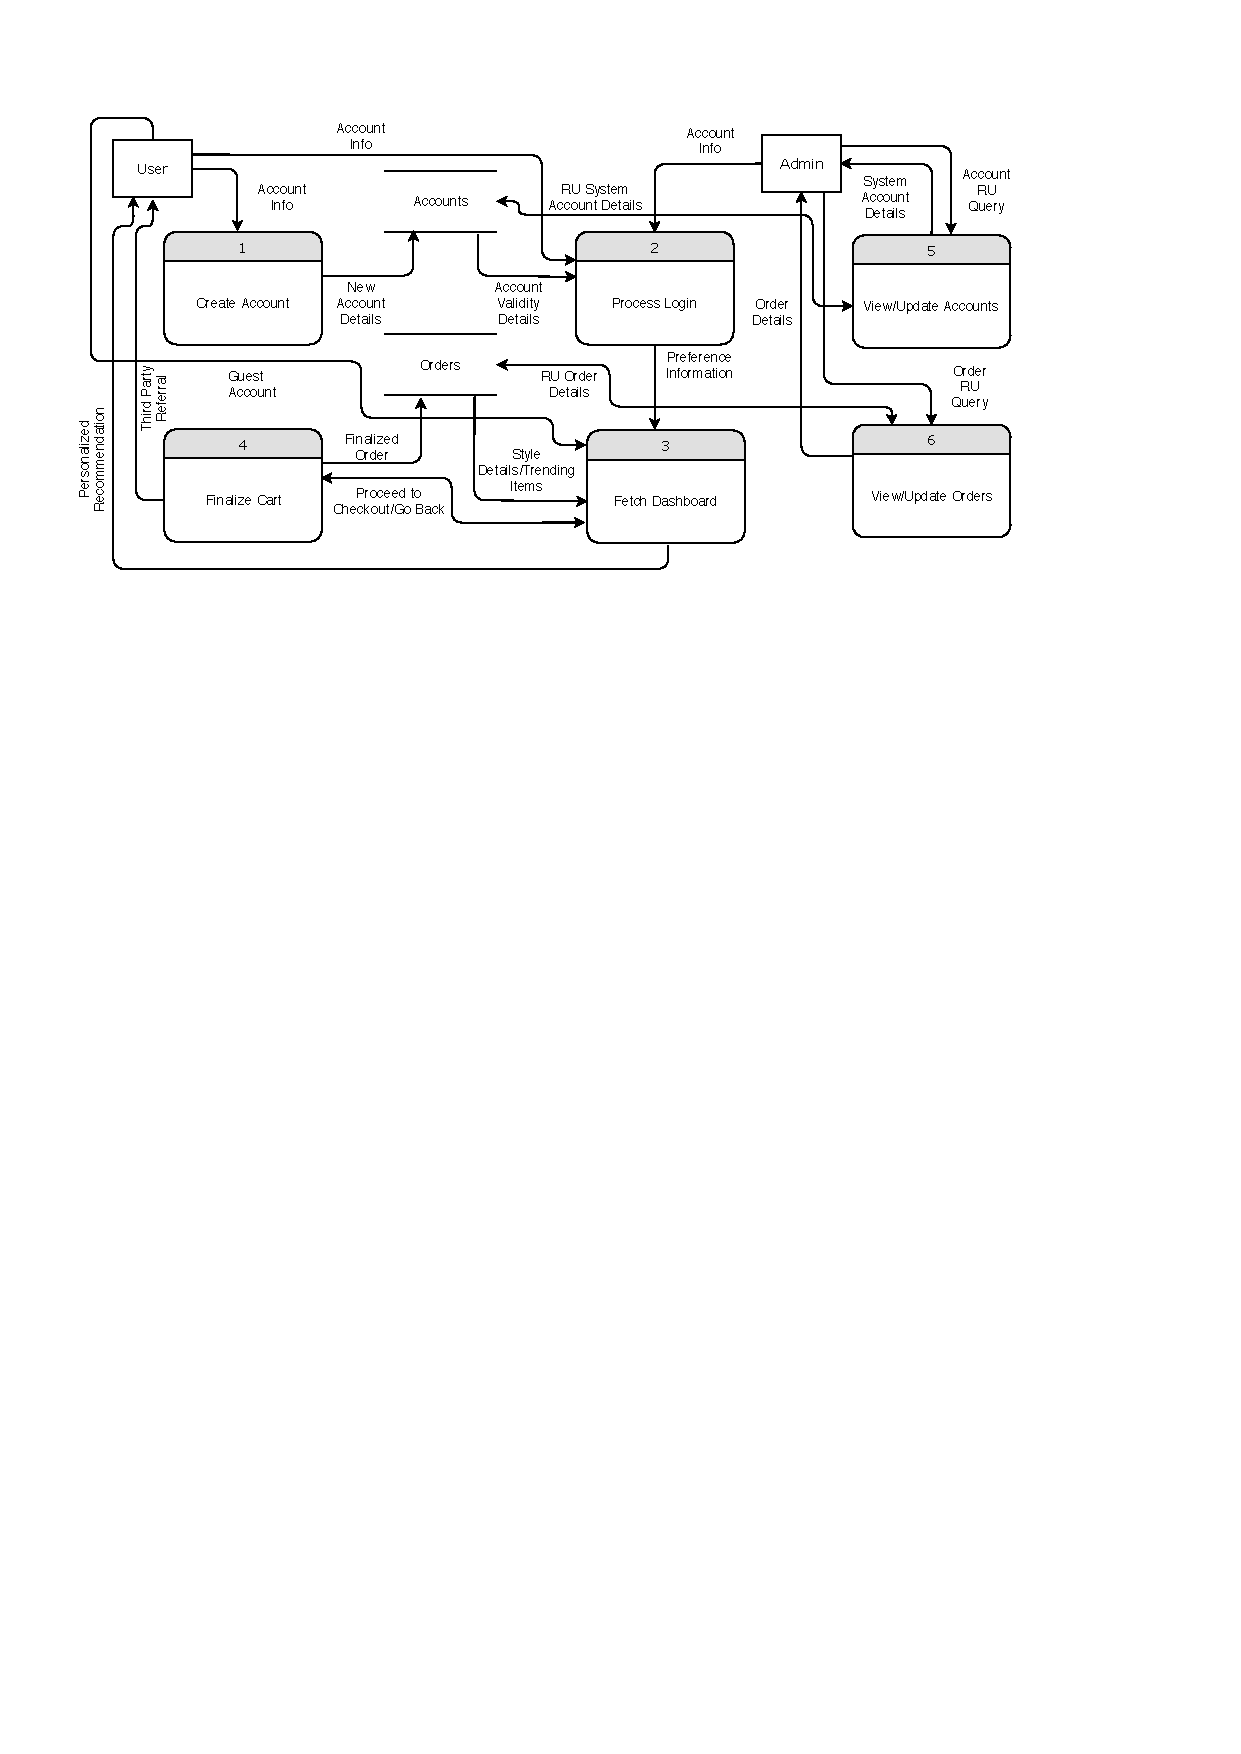
\includegraphics[width=15cm]{images/dfd0.pdf} 
\centering
\caption{0-Level DFD}
\label{dfd:zero}
\end{figure}

\section{Association Matrices}
Association matrices for the system are depicted in \autoref{crud:dToL}, \autoref{crud:dToP}, and \autoref{crud:pToL} ahead.  
\begin{table}
\centering
\begin{tabular}{ |c|c|c|c| } 
\hline
 & User & System Admin \\
\hline
\textbf{User} & Individual & All \\ \hline
User ID & R & CRUD \\ 
Name & RU & CRUD \\ 
Email ID & CRU & RD \\
Password & RU & RD \\
\hline
\textbf{Sign in/Sign up/ Sign out} & Individual & All \\ \hline
Account ID & R	& RD \\ 
Date &	R	& RD \\
\hline
\textbf{Verify Credentials} &	Individual	& All \\ \hline
Account Valid &	R &	CRUD \\
Logged In &	R &	CRUD \\
Date &	R &	CRUD \\
\hline
\textbf{Fetch Dashboard} &	Individual &	All \\ \hline
Page ID	& R	& CRUD \\
Image Details &	R &	CRUD\\ \hline
\textbf{Finalize Cart} &	Individual	& All \\ \hline
Cart ID	& R & CRUD \\
Date &	R &	CRUD \\
Item No. &	RU & CRUD \\
Third-party Referral &	R & CRUD \\ \hline
\textbf{Recommendation Details}	& Individual &	All \\ \hline
Recommendation ID &	R &	CRUD \\
User ID	& R & CRUD \\
Date &	R & CRUD \\ \hline
\textbf{Image} &	Individual	& All \\ \hline
Image ID &	R	& CRUD \\
Category & R & CRUD \\
Image Attribute	& R &	CRUD \\
Recommendation ID &	R &	CRUD \\ \hline

\hline
\end{tabular}
\caption{CRUD: Data to Location Matrix}
\label{crud:dToL}
\end{table}
\begin{table}
\centering
\begin{tabular}{ |c|c|c|c|c|c|} 
\hline
 & Account  & Credentials	& Dashboard & Cart & Image  \\
\hline
\textbf{User} &  &  &  &  & 5  \\ \hline
User ID	& R & R & R	& R &	R \\
Name &	CRU	& RU & & & \\	
Email &	CRU & R	& &	& R \\
Password &	CRU & R	& & & \\ \hline
\textbf{Sign in/up/out} & & & & & \\ \hline
Account ID	& R	& R & & & \\
Date &	R &	R & & & \\ \hline
\textbf{Verify Credentials} & & & & &\\ \hline		
Account Valid & & RU &	R &  & \\		
Logged In & & RU & R & & \\		
Date &	& R & R & & \\ \hline
\textbf{Fetch Dashboard} & & & & & \\ \hline		
Page ID	&	&	& R	& R & \\ 	
Image Details & & &	RUD	& RU & \\ \hline
\textbf{Finalize Cart} & & & & & \\ \hline		
Cart ID	&	& 	& R	& R & \\	
Date &	&	&	R &	RUD	& \\
Item No. &	&	&	R	& RUD & \\	
Third-party Referral &	&	&	R	& RUD & \\ \hline	
\textbf{Recommendation Details} & & & & & \\ \hline
Recommendation ID & & &	R	& RU & \\	
User ID	&	&	& R	& RUD & \\	
Date &	&	& R	& RUD & \\ \hline
\textbf{Image} & & & & & \\ \hline	
Image ID & & &	R & R & R \\ 
Category & & & RUD	& RUD & R \\
Image Attribute & & & RUD	& &	R \\
Recommendation ID & & &	R & R & R \\ \hline
\end{tabular}
\caption{CRUD: Data to Process Matrix}
\label{crud:dToP}
\end{table}

\begin{table}
\centering
\begin{tabular}{ |c|c|c| } 
\hline
 & User & System Admin \\
\hline
Process Account & * &  \\ \hline
Process Verify Credentials & & * \\ \hline
Process Dashboard &	 &	* \\ \hline
Process Cart &	*	&  \\ \hline
Process Image Handling &  & * \\ \hline
\end{tabular}
\caption{CRUD: Process to Location Matrix}
\label{crud:pToL}
\end{table}